% Todo:
% * Change self-pic
% * Guns Germs and Steel explain a bit more
% * Americanism explain a bit more
% * "It is not humanly bearable" -- Hanasaki
% * "I wish you happy" -- Cate

\documentclass[12pt]{report}
\usepackage{color}
% \usepackage[dvipsnames]{xcolor}
\definecolor{SmurfBlue}{rgb}{0.0,0.25,0.85}  % Smurf Blue
\usepackage[unicode,colorlinks=true,linkcolor={SmurfBlue},
	pdfauthor={YKY},
	pdftitle={Paranoia},
	pdfsubject={auto-biography},
	pdfkeywords={biography, mental illness, racism}
	]{hyperref}
\usepackage[no-math]{fontspec}
%\usepackage{CJKutf8}
\usepackage{xeCJK}
%\setCJKmainfont{ukai.ttc}
%\setCJKmainfont{gkai00mp.ttf}
%\setCJKmainfont{KaiTiM}
%\setCJKmainfont{SimSun}
%\setCJKmainfont{FangSong}
\setCJKmainfont[BoldFont=SimHei,ItalicFont=SimSun]{SimHei}
% \setCJKsansfont{SimHei}
% \setCJKmonofont{SimKai}
% \usepackage[default]{droidserif}
% \usepackage[T1]{fontenc}
\usepackage{gensymb}		% for \degree symbol

\usepackage{cite}
\usepackage{graphicx}
\usepackage{float}
\usepackage{amsfonts}
% \usepackage{amsmath}	% for \tag
\usepackage{amssymb}	% for \multimap
% \usepackage{stmaryrd}
%\usepackage[square,numbers]{natbib}
%\nocopyright
%\usepackage{latexsym,amsmath,amssymb,graphicx,hyperref}
%\usepackage{times} % gives you a bit more space if needed
\usepackage{titlesec}		% change color of section headings
\usepackage{verbatim}
\usepackage{pdfpages}		% book cover
\usepackage{framed}			% title page's box
\usepackage{datenumber,fp}	% for year calculations
\usepackage{accents}		% for dots under Chinese for empahsis
\usepackage[nohints]{minitoc}		% mini table of contents
\usepackage{caption}		% suppress caption numbering
\usepackage{tikz-cd}		% commutative diagrams
\usepackage{setspace}		% reduce line spacing for code
\usepackage[normalem]{ulem}	 % such that \underline won't overflow
\usepackage{lastpage}		% get total number of pages
% \usepackage{movie15}		% for reaction-diffusion movie ("History" chapter)
% \usepackage[dvipdfmx]{movie15_dvipdfmx}
\usepackage[dvipdfmx]{movie15}
% \usepackage{media9}		% Doesn't work for Linux Acrobat Reader

\xeCJKsetup{CJKecglue = {\hskip 0.1em plus 0.02em minus 0.01em},
  xCJKecglue = {\hskip 0.1em plus 0.02em minus 0.01em}}

% Omit chapter number in equation numbering
\renewcommand{\theequation}{\arabic{equation}}
\renewcommand{\familydefault}{\sfdefault}	% use san-serif font

\definecolor{Magenta}{rgb}{0.4,0.1,0.4}  % Magenta
% \definecolor{LogicColor}{rgb}{0,0,0}	% for black-and-white paper

\titleformat{\chapter}
{\color{SmurfBlue}\normalfont\huge}
{\color{SmurfBlue}\thechapter\\}{1em}{\flushleft}

\titleformat{\section}
{\color{SmurfBlue}\normalfont\large\bfseries}
{\color{SmurfBlue}\thesection}{1em}{}

\newcommand{\code}[1]{\texttt{\textcolor{Magenta}{\small{#1}}}}
\newcommand{\tab}{\hspace*{1cm}}
\newcommand{\concept}[1]{\textbf{\textcolor{blue}{#1}}}
\renewcommand{\textbf}[1]{\textcolor{red}{#1}}

% Make dots under Chinese characters for emphasis
\renewcommand{\d}[1]{$\underaccent{\scalebox{0.5}{\textbullet}}{\textrm{#1}}$}
\makeatletter
\newcommand{\ds}[1]{%
  \@tfor\next:=#1\do{\d{\next}}}
\makeatother

\newcommand*\sadface{\includegraphics[scale=0.25]{face-sad.png}}
\newcommand*\smiley{
\includegraphics[scale=0.5]{smiley.jpg}}
%\newcommand*\vignette{\centering{\color{blue} --- \quad $\diamond$ \quad --- \quad $\diamond$ \quad --- \quad $\diamond$ \quad --- }\par}
%\newcommand*\vignette{\begin{center}\color{blue}  --- \quad \S \quad --- \quad \S \quad --- \quad \S \quad --- \end{center}}
%\newcommand*\vignette{\begin{center}
\includegraphics[scale=0.5]{vignette1.jpg}\end{center}}
\newcommand*\todo{\begin{center}\color{red}  \rule{5cm}{0.5pt} 以下是草稿\, \rule{5cm}{0.5pt} \end{center}}
\newcommand*\dashh{\textemdash\,\,}

%%%%%%%%%%%%%%%%%%%%%%% vignette command %%%%%%%%%%%%%%%%%%%%%%%%%%%%%%
\makeatletter
\newcount\sk@vignette
\newcommand*\vignette[1][]{\begingroup
\ifx\@empty#1\@empty
    \global\advance\sk@vignette by\@ne\relax
\else
    \sk@vignette=#1\relax
\fi
\ifnum\sk@vignette>18\relax
\sk@vignette=\@ne\relax
\fi
\begin{center}\includegraphics[scale=0.5]{vignette\the\sk@vignette.jpg}\end{center}
\endgroup}
\makeatother

\setlength{\oddsidemargin}{0cm}
\setlength{\evensidemargin}{0cm}
\setlength{\textwidth}{16.5cm}
\linespread{1.3}

%%%%%%%%%%%%%%%%%%%%% count number of words
\immediate\write18{./count-words.sh}

\begin{document}

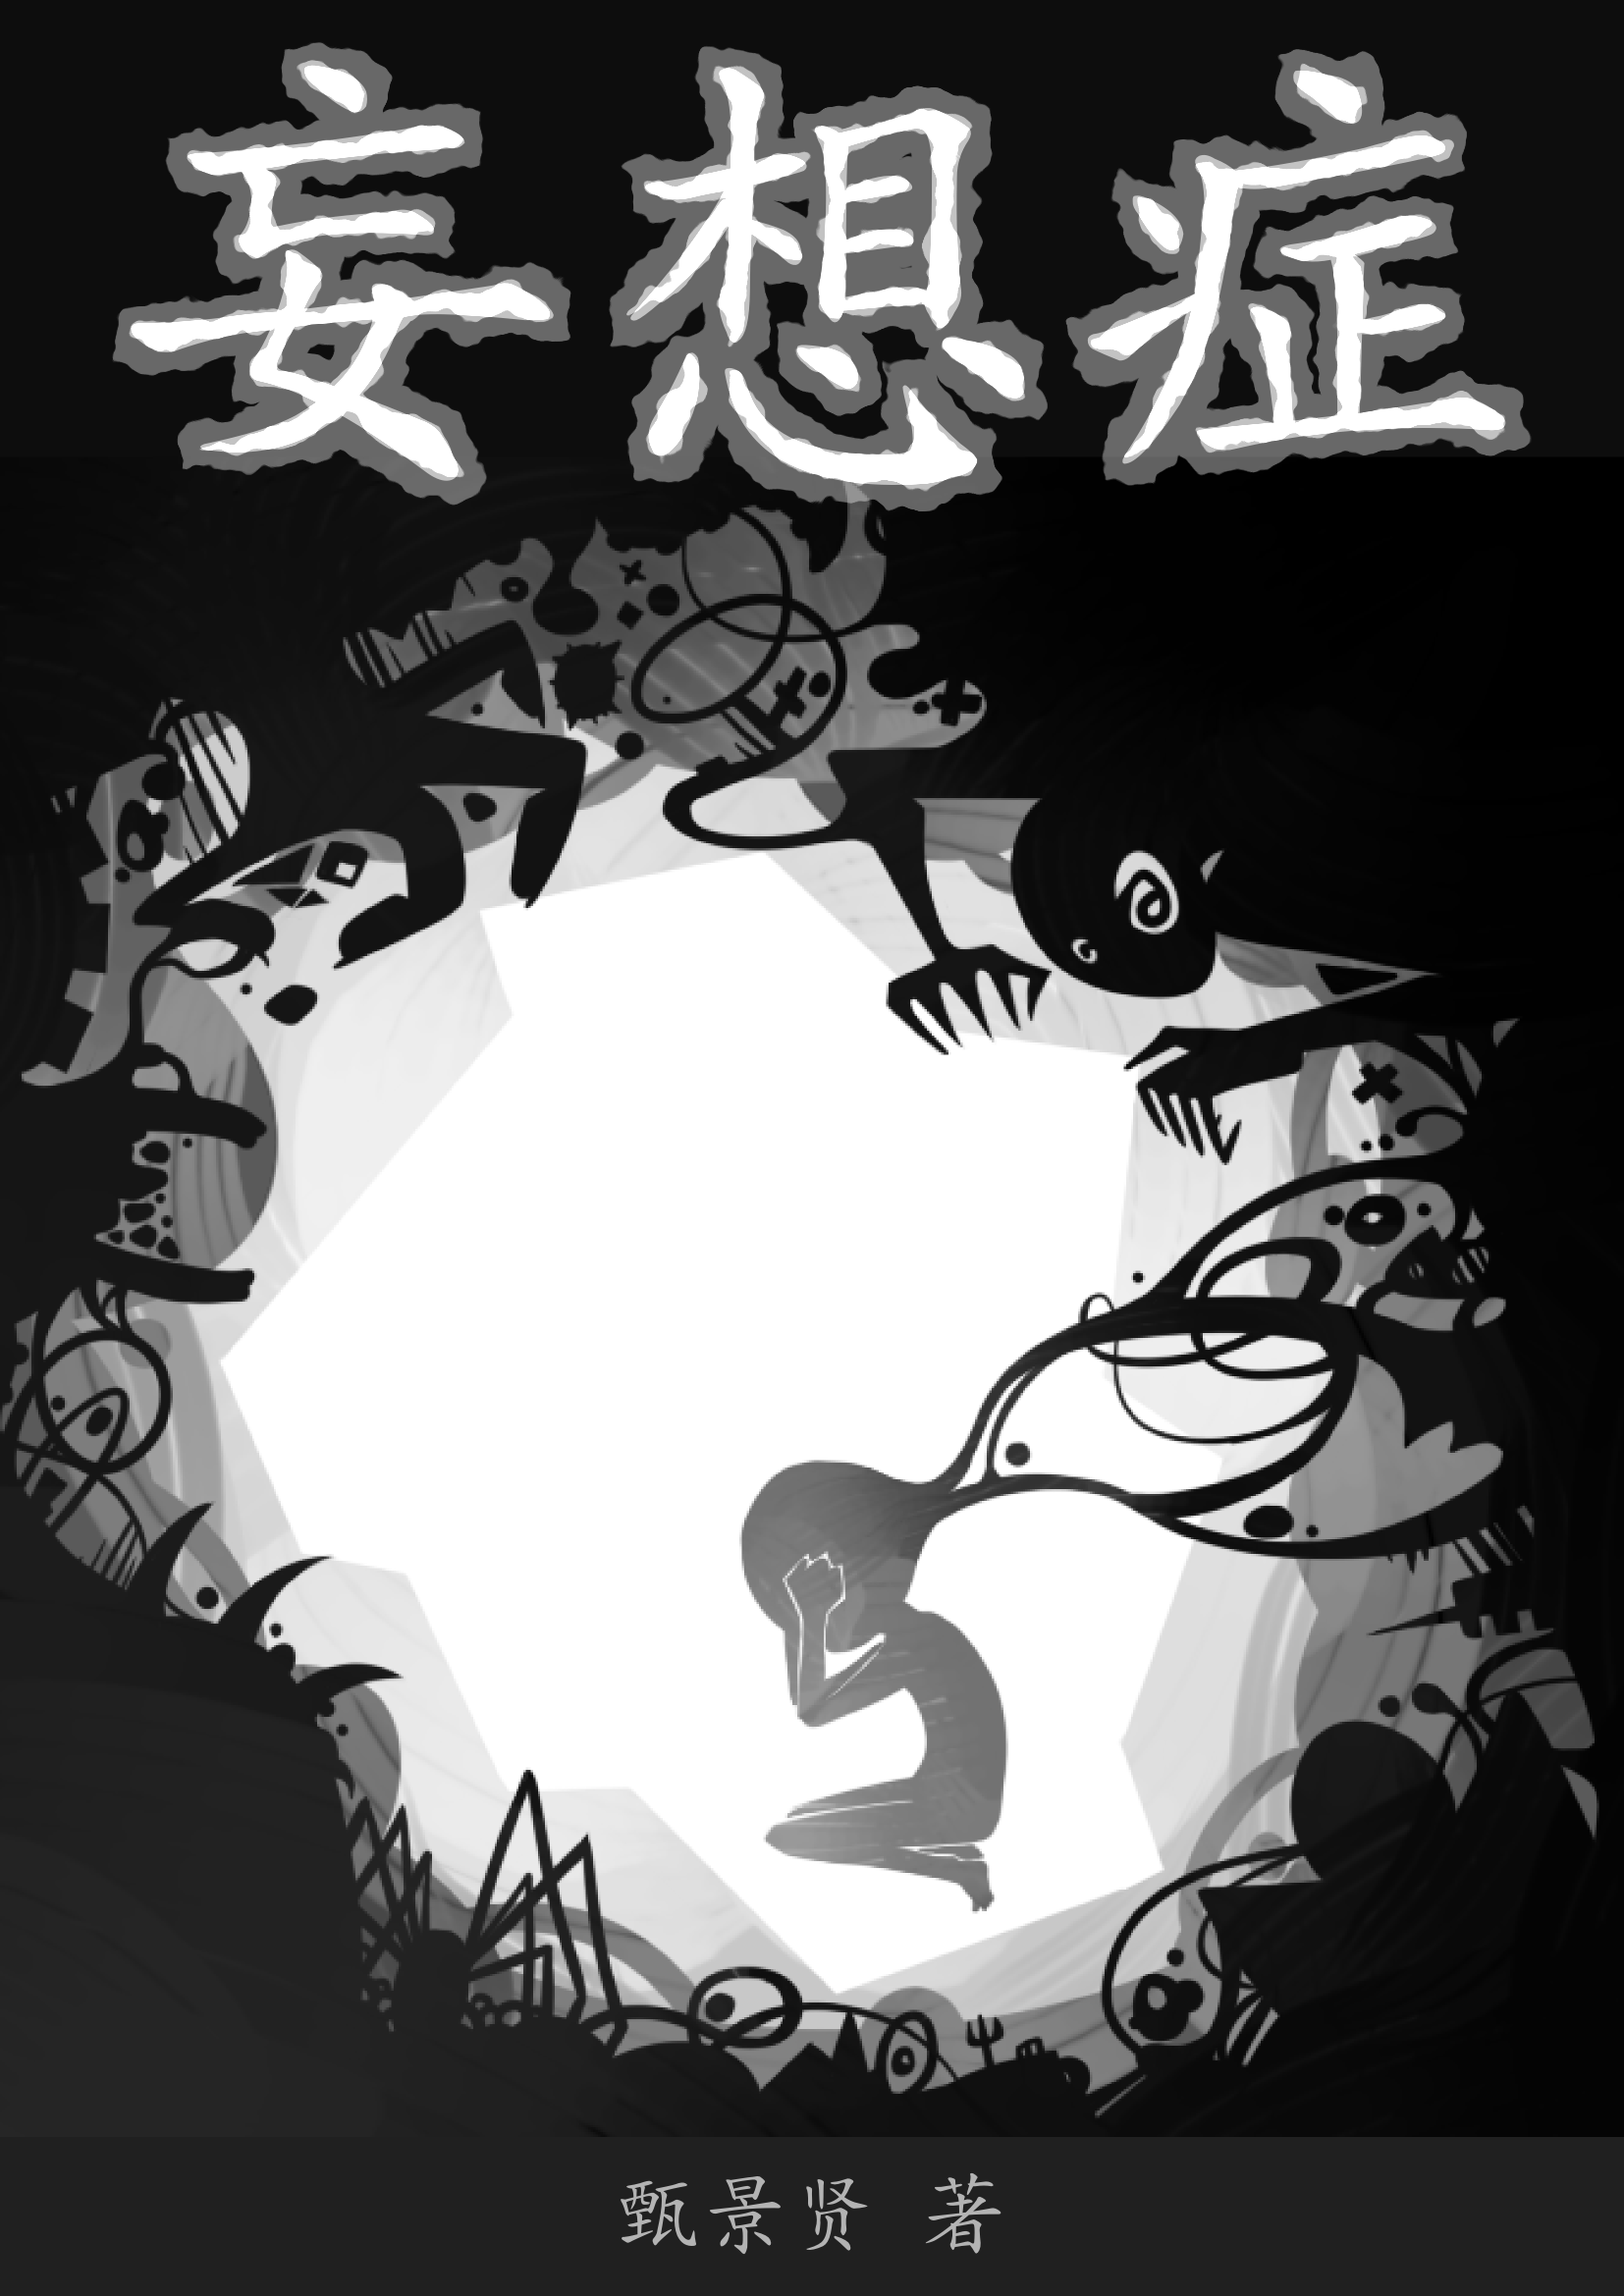
\includepdf[fitpaper=true]{cover1-mong}
\cleardoublepage
\title{\Huge{妄想症}}
\author{YKY (甄景贤)}
% \date{27 May 2015}
% \institute{}

% Calculation of some years
\newcounter{dateone}
\newcounter{datetwo}
\newcounter{datezero}

\setmydatenumber{dateone}{1991}{08}{01}		% Cousin visit HK in summer
\setmydatenumber{datetwo}{1996}{09}{01}		% first arrive in USA
\setmydatenumber{datezero}{\the\year}{\the\month}{\the\day}

\FPsub\resulta{\thedatezero}{\thedateone}
\FPdiv\resultb{\resulta}{365.2425}
\FPround\resultb{\resultb}{0}

\FPsub\resultc{\thedatezero}{\thedatetwo}
\FPdiv\resultd{\resultc}{365.2425}
\FPround\resultd{\resultd}{0}

\large

{\let\newpage\relax\maketitle}

\maketitle
\setlength{\parindent}{0em}
% \setlength{\parskip}{2.8ex plus0.8ex minus0.8ex}
\setlength{\parskip}{2.8ex}

\small

\begin{framed}
这本书的起源是回答《知乎 www.zhihu.com》网站的问题『精神分裂症患者眼中的世界是什么样的?』 ~很多地方写得不好,但我想尽快发表这个草稿,以后还会修改和添补。

欢迎读者们提问或提供意见: general.intelligence@gmail.com

字数: \input{word-count.txt}  ~~~\pageref*{LastPage} 页

封面插图:  谢谢 Nami-Tsuki (Jessica Allen) 的画作 ``Paranoia or something'', DeviantArt.com
\end{framed}
\large

\newpage

\tab\tab\tab \parbox{9cm}{\textit{Love is an act of endless forgiveness,\\
a tender look which becomes a habit}}
\vspace{0.5cm}
\begin{flushright}
\dashh Peter Ustinov \hspace*{3cm}
\end{flushright}

\vspace{3cm}

\begin{center}
{\Large 内容撮要}\par
\vspace{0.5cm}

\parbox{0.8\textwidth}{
本书主要围绕两个问题:\par

\begin{enumerate}
\item 究竟堂妹有没有骗我? 还是我恼羞成怒? 我为什么怒到想杀了她? 
\item 究竟是我有精神病,还是香港人/美国人都错了?
\end{enumerate}

希望聪明的读者能帮我解答这些问题。
}
\end{center}

% \dominitoc
\tableofcontents

\chapter{妄想症}

我有 persecution paranoia (逼害妄想),特别地叫 Truman Show syndrome。 在《Truman Show》这部 1998 年的电影里,主角活在一齣真人表演里,他身边的人都是演员,但从小欺骗着他,最后他走出了这个骗局。 在外国有很多人有这种妄想,多到形成了症候群的名字。

我 25 岁时 (1996 年) 初到\uline{美国},那时迷恋我的\uline{美国}堂妹但遭拒绝。 再加上在外国生活和很少朋友, 而且我从小便对白人的种族歧视很有反感,所以觉得自己活在充满敌意的环境里。 这些因素,令我到了\uline{美国}不够一年便产生了 Truman Show 妄想。 (起初是怀疑有人偷看我的电邮开始....)

\resultb 年后的今天,我其实仍然未「康复」。 我现在打这篇文章,我的脑子一半觉得自己独自在房间里打字,一半觉得是在全世界 Truman Show 的众目睽睽下打字。

你可能觉得我疯了,为什么像 Truman Show 那样荒谬的情节,都会觉得是真的?

我正在研究人工智能,这个技术在不久将来可能会颠覆世界秩序。 例如,白人和有色人种的主要分别,可能只是外貌上的不同,但这外貌是由基因遗传的,我们\uline{中国}人不能拥有那些基因,除非强抢他们的女人来交配。 有人工智能后,技术的发展可使人长生不老,那时候人类会脱离基因的约束,我们想变什么模样都可以。 而白种优势 (white supremacy) 也将会随之消失。

所以,西方人可能不想让\uline{中国}人掌握这技术。 而我确实遇到了来自\uline{美国}的人工智能研究者的排斥:他们叫 OpenCog,创始人是 Ben Goertzel,他现在颇有点名气,你可以上网查查。 我试过很多次想加入他们,但他们态度很不友善、诸多阻挠。

所以,如果我觉得\uline{美国}或西方有人想害我,其机率实在未必是零。 你不见有很多反\uline{美}的政治人物都被害死了? 而我的立场是坚决反对种族歧视,在逻辑上必然导致要反\uline{美}。

原本想找个代笔的人帮我写书,但慢慢的我把想写的基本上都写了。  有机会还会翻译成\uline{英}文。

住过精神病院 3 星期,在那里见过一些人和事,很同情他们。 我被吓得半死,装着正常求他们放我,终於在圣诞节那天他们放了我出来,使我想起 《One Flew Over the Cuckoo's Nest》\footnote{《飞越疯人院》(1974)}这齣戏 (戏中的正常人被电击至白痴,而那以为自己是\uline{耶稣}的人却成功逃离)。 戏中还教人把药藏在脷底下,想不到这点小知识后来对我很有用。

关於那些精神科药物,它们是没有帮助的,只是把神经传播的讯号分子阻碍 (blocking),会导致人嗜睡、没精神、失去动机 (motivation)、性欲等。 男孩子还会变女性化。 说得简单点就是用药物把脑部部份切除 (虽不是永久性的)。 我因为先前研究过如何将人脑的「意识」上载到电脑上 (mind uploading),所以对神经科学很熟悉。 信我吧!

\uline{甄景贤}是真名 —— 为什么用真名? 因为我有一半认为,你们已经知道这一切了 \smiley

\chapter{殖民主义}

我爸以前在\uline{香港}当皇家警察的,\uline{香港}回归\uline{中国}后他继续做了几年才退休。 我年轻时从没有因为父亲的职位觉得不妥,但到了\uline{美国}后就开始强烈地意识到了。 毕竟,为殖民主义服务,是卖国的一种形式。 奇怪的是,在\uline{香港},大部分人压根儿不觉得殖民主义可耻。 有人甚至认\uline{英国}政府是「契妈」、比生母还要亲。 为什么这样呢? 殖民时期的\uline{香港}虽说是个「华洋杂处」的地方,但其实西人对华人来说,仍然是「高不可攀」的 (这情况或许正在改变),有很多\uline{香港}人提到要讲\uline{英}语便会脚软。 在这种恐惧之下,他们不能正确地认清殖民主义的真面目。

我接触\uline{美国}后,有好几年都完全被他们的进步文明慑服了,就像小\uline{布殊}说的 ``shock and awe'' 那样。 有时期连中式食物都不敢吃,要吃全西餐。 但后来回到\uline{香港},在报纸上看到「西方伪善\footnote{western hypocrisy}」这个术语,从此对国际间发生的事,真是豁然明白了很多。

小时,我有个阿姨,去了\uline{英国}念文学。 我见她不多,印象中就只有一次她对我们忆述在\uline{英国}念书的情景,说有一次集体用餐时,她伸手拿面包,有\uline{英国}男生对她说 ``don't touch that bread!'' 那样的话。 (确切的那句话不记得了,总之是叫她不要碰那面包,应该不是叫她吃高纤面包吧?) 后来她在\uline{香港}的一间 Islam 中学教书,得了白血病死了。 在我想像中,觉得她是个自尊心很强的人 (在外婆的女儿中,她大概是最漂亮的,学历也最高),因被人歧视而在郁结中死去。

\chapter{世界 A 和世界 B}

自从思觉失调之后,我无法分辨这个世界究竟是世界A (现实) 还是世界B (真人秀)。 在地铁看见别人窃窃私语时,不知道她们是不是在谈论我。 总觉得\uline{香港}和\uline{美国}的电视节目在含沙射影地嘲讽我,有时又用肥皂剧的角色映射我、咀咒我死掉; 这些都令我极之讨厌。 但我又无法分辨世界 A 和世界 B。 换言之,我已经变成了一个盲人,就像《圣经》\footnote{我是无神论者,但圣经里的故事有时是很有意思的。}里 Samson 和 Delilah 的故事:Samson 被她出卖之后,被人剪去头发和弄盲了,从此他的努力工作都是\ds{徒劳无功}的,变成了他的敌人的笑柄。 我常常觉得,我当初和堂妹的纠缠,就是解开这一切问题的关键,所以不停地分析那段日子。 那时候思想和感情都很混乱,是走上疯狂之路的开端。

首先要釐清的是,我虽然迷恋她,但其实也看不起她、也有想要别的女孩,而我我像遇难的船客掉进了\uline{太平洋},像抓着救生圈那样缠着她不放。 因为她是 ABC\footnote{American born Chinese},她是一张打入白人社会的入场券,能娶到她该多好啊,否则就像漂浮在大海,徬徨着不能「上岸」。

终於在\uline{纽约}见到她,她已经明显不喜欢我。 那时我带来了一本书,是一个\uline{加拿大}华裔女孩写的,讲她离家出走后卖淫的自传式小说,我知道女孩子没有不喜欢那种书的,果然我把书遗在伯娘家,然后她两姊妹都看了。 书还回来后,竟然有堂妹的笔迹写的小纸条,就只写了一句 ``no escape except through death''\footnote{『没有出路,除非通过死』}。 那时我觉得她是在耸恿我去把我的某个中学朋友杀掉。 (因为堂妹最初跟伯娘到\uline{香港}旅行,那是我最初喜欢她的时候,我把那中学朋友介绍给她,原以为大家可以一起开心玩,没想到他俩眉来眼去,把我变成傻子一样。) 我越来越觉得那是奇耻大辱,非要杀他报仇不可 (就像一把插在我和堂妹之间的剑,一定要拔掉),但自己又身陷真人秀里,怎能杀人? 而且,堂妹若真的爱我,怎会要我杀人为条件? 当初不是他俩在调情才做成这耻辱吗? 每想到这里就愤怒到浑身发抖。

十几年后,最近终於好像明白了她那句句子的意思。 其实在\uline{美国}文化里,最高级的人是金发蓝眼的;如果红头发的话,是不祥的;如果黑头发,那么她们触摸的一切都会变成悲剧。 至於\uline{犹太}人更不用说了,把卷曲的头发烫直再说吧。 而黄种人比\uline{犹太}人更低级。 我妒忌我的\uline{美国}堂妹比我「先上岸」,仿佛她先过我变成了白人,我妒忌到想把她杀了,而我以前从来未对人怀过那么深的怨恨。 而其实,这个所谓「上岸」指的是什么? 所有\uline{美国}华侨,在\uline{美国}只不过过着次等的、没有尊严、像影子一般的 existence。 就算 Whitney Houston\footnote{(1963-2012) \uline{美国}黑人女歌手,她的歌词里叫人要懂得自爱,不要活在别人的影子下,我中学时老师播给我们听。} 都不过是个影子,\uline{奥巴马}更干脆背叛了自己黑人的那一半,他还 cool 到露出微笑。  注意:\uline{乔布斯}\footnote{(1955-2011) 苹果电脑的创始人}就是一个「认继父母不认亲父母」的人。 在\uline{美国},有色人种越来越绝望,甚至当妓女贱卖,那些白人男孩都未必会揪一眼。 谁都上不了岸,我们在海难中互相拉扯,丑态百出。『除死以外没有出路』可能就是这个意思。

\chapter{American cousin}

1991 年(\resultb 年前),来自\uline{美国}的伯娘和两个堂妹来\uline{香港}旅游。 我 20 岁,刚进大学二年,堂妹 14 岁。

那时候家里很热闹,来自\uline{英国}的表弟也和一个白人朋友来\uline{香港}旅游,所有人都住在我家。  堂妹她们到达的那一晚,我刚从大学宿舍回来,她们已经进房睡了,妈在客厅中低声向我「汇报」描述这些新来的客人。    她面带愁容地说: 哎吔.... 那两个堂妹的打扮很「吓人」.... 那个大的痴肥,身体像座山那样; 那个小的,年纪轻轻已经涂指甲、口红、香水,像个「老人精」。   我听了之后心里已经很喜欢她; 这些故事从来就是这样开始的。

相识还不够一天,堂妹说:「堂兄妹也可以结婚,如果不生孩子的话。」 我故意面色很凝重地点头。

5 年后,痴情的我到纽约找她,她说她已有男友,她要结婚生孩子,我们不可能。 我和她纠缠,我说她不给我合理解释; 她说我像个 psychopath (神经病人) 很可怖。 而我当时的确开始了被人监视的妄想 (她不知道); 我很想和她谈的原因之一就是想她帮我弄清有没有被监视的问题 \dashh 甚至她也可能是观众之一?

其实 1991 年那暑假,初相识的几天之后,她已经换了态度,说:「我只想要个哥哥,把欺负我的人揍一顿。」 我当时的反应是:「Huh? 揍谁?」

\resultb 年来我不停思索为什么她嫌弃了我。

14 岁的她说:「(老)\uline{布殊}在\uline{伊拉克}打仗,他还一边打高尔夫球!」 我说我们香港人不问政事,不知什么叫打仗,与及一些类似的蠢话。  现在我明白到,她说的很对,她年纪小小已经很懂事。  现在我知道正确的答案,是我们应该要打倒\uline{美国}的帝国主义和种族歧视。

\vignette

在\uline{纽约}的大学宿舍,正对着窗前是一颗大树,春天时,树上的一对鼬鼠 (?其实我也不清楚它是什么动物)天天在追逐。 大概是发情期吧,那雄性鼬鼠老是朝着雌性的尾部追去,但又总是追到贴近尾部 却又揽不住她,看起来就像只是为了嗅那气味,看得我直冒火。  我只身来到\uline{纽约},但堂妹不想见我,我们当时的处境分明就像那两只在追和被追的鼬鼠,我觉得那境象简直令人眼冤,就像拉粪和放屁的生理现象那样讨厌。  想起一本小说的名字: The Heart is a Lonely Hunter。  想起电影中理想的情侣、「青青珊瑚岛」、在花间嬉戏、女的含情脉脉地看着男的,那景象和我的现实截然不同。  我是在追者,她是在逃者,但青青珊瑚岛的他俩是两情相悦的。  一定有什么出错了,但又想不出是什么原因;~ 感觉一切都和我作对,everything is against me。  \uline{莎士比亚}说:世界是舞台,我们是演员,而我发觉我这「在追者」的角色是一个根本不可能演得好的角色。  我一步也不可以追,一追就错了,但我已经在追了。

我又想起一齣电影: 年青人的漂亮妻子被敌人胖子看上了,他们互相赌博,年青人把身家输光了,把妻子也拿来赌。  当然最后还是年青人赢了。  在那结尾的一幕,他把妻子赢回,而胖子啕哭起来,那女的用手揉他的背 ~安慰他。  为什么这角色降临到我身上?

我又想起有一次在地铁里,有个母亲当着其他乘客的面在规教小女孩,而那小女孩用手掩着耳朵不听,似乎很懊恼她母亲把她的糗事公诸於世。  当时的我就像那小女孩,不想听到真相。

我心里产生一幅图像: 我没有穿衣服,黄色皮肤的身体像只低等动物,我很拙劣而原始地,用手捏着泥巴,在筑一道小围墙,想把堂妹围进我的世界里,而那围墙矮矮的细小得可怜,只够围着我自己一人,里面的环境污糟邋遢,而我堂妹居高临下看着我,我还懵然不知。  我越来越觉得这个泥塔无法经营下去,真相像四面\uline{楚}歌那样迫过来。  终於,我抬头看见堂妹在看我,我恼羞成怒,想骂她:『妳明知不会喜欢我,为什么不早点告诉我?』  然后又想起: 她岂不是一直反覆告诉我她不喜欢我,而我却莫名其妙的听不进去?

我又想,所有人在成长的过程中都要经过失恋的痛苦,为什么我搞得特别糟糕?  很多旧同学也大学毕业了、结了婚、生了孩子,没听过他们闹出什么丑闻。  为什么别人适应良好,难道是母亲以前教漏了什么?   为什么教科书上没有?   也有一个旧同学,他在大学宿舍爬墙偷看女朋友的房间,发现她和另一男孩偷情,还摔下去跌断了腿。   他正是上面我提过的,和我堂妹眉来眼去那人。

有一晚在宿舍里,我鼓起勇气打电话给她,但又害怕,电话的听筒拿起了又放下,拿起了又放下.... ,最后还是打了给她。 她问我『你想说什么?』   而我说:『我... 我... 我... 』那样重复地口吃着那「我」字,真的有一兩分钟之久。  因为我觉得心虚,我不是真的爱她,而是因为得不到她,所以想征服她。  我觉得我对她的爱不是真的,我分明瞧不起她,但又很怕被她识破。  我不会为她而死,甚至我能肯定地预测到,如果追到她以后,我也会喜欢别的女孩。  那就像一场真心的比拼,而我心虚了,最后我说:『我... 我... 我... 很爱妳 。』  她好像觉得受了冒犯似的,狠狠地挂断了电话。

后来我在网上和一个\uline{美国}女人谈起这件事,那女人态度有点傲慢,她说: ``So she's smart .... Forget her and move on.''  但我越来越怀疑,虽然女人经常看爱情小说,但其实女人是不是真的比男人更懂爱情?

我想起,其实她似乎也喜欢很多别的男孩。 在她14岁那个夏天,我们不知怎地聊到性的话题。  我理所当然地说:「我喜欢很多种类的女孩,但妳是女孩,妳当然只会和妳真正喜欢的男生才做爱。」 可是她说:「不啊,我跟谁都做!」 我被她突如其来的反驳搞得很不知所措,而且很害怕她会和别人做爱。 我安慰自己说,她一定是说笑而已....

等公车的时候不见公车,不等的时候却遇见很多。  在\uline{纽约}单恋堂妹的时候,特别多女生勾引我。 但我那时故意不睬别的女生,以表示我对堂妹有多忠心。  其实那只是我一厢情愿地想找些理由逼她喜欢我。  在大学上课时,有个女生在后面丢了笔到地上,而我居然全身绷紧了不去帮她拾,因为我怕是她在勾引我。  我甚至隐约听到那女生很惊奇地低声说 ``what?'' 然后她自己拾回那笔。

\vignette

在\uline{纽约},她的 (不是男友的) \uline{美国}朋友 Ralph 对我动手动脚,警告我不要再骚扰堂妹。 我没有还手,当时的我实在搞不清发生什么回事。 然后我跟伯娘投诉堂妹为什么不给我解释,打了伯娘一下。 伯娘打电话招援,我被他们一众亲戚朋友打了一顿。 我说 Ralph 先动手打我,但我不知他们接收到没有。

被打一顿之后,我跌坐在房子外的草地上,手臂在流血(但只是皮外伤)。  伯娘指着我痛骂:「你这算读什么书? 读屎片!?」 过后又写了张支票给我,也许是作为「失恋补偿」?  这次事件后我和她们很少见面了。

那天伯娘本来为了帮我搬家,特意从老远驾车到我住处,但我不感激她还觉得她们欠了我。 我那时处於人生的极低点,真是 inconsolable.

伯娘以前已经和我解释过:『如果她真的喜欢你的话,不会是这样的』、『你若不服气,将来努力点,胜过她。』 其实她的话很有道理,我听了之后真的很努力发奋。

\resultb 年后的今天,我看见那些软弱无能的\uline{香港}人,有无法抑制的想朝他们面上揍一拳的冲动,觉得不教训实在不成体统。 但那岂不是等於打 \resultb 年前的我自己?

我妒忌堂妹,因她父母先到\uline{美国}移民,她们很早便认识到外国人的 尔虞我诈 和 aggressiveness (侵略性),但外国也比我们进步很多,而我只是\uline{香港}来的驯良的乡下仔。 我很愤怒,为什么是个小丫头教训我,但我想不出有什么可批评她(除了一些琐事)。

但其实她也有缺点,也是个普通人。 14 岁的她也说过一些蠢话,蠢到笑死人。 想不想听? 例如她说 :「我以前不信有鬼,但看了《Ghost》\footnote{《人鬼情未了》(1990)} 这齣电影后我真的信了。」 那个主演的 Patrick Swayze 现在真的变了鬼。

她又好像很好心地告诫我:「\ds{不要信任何人}!」 回想起来, 她的一句话,和我被那中学朋友出卖等事,真的令我什么人都不信了。 而彻底怀疑的结果就是我连所有人是不是在演戏都分不清,甚至包括她在内。

初相识的时候,我常为小事对她说「对不起」,但她说:「不要老是 say sorry,我最讨厌人说 sorry」,而我在她面前真的常常觉得自己笨头笨脑。  她走之后我发了神经,无论什么情况都不对人道歉。  在\uline{纽约}的大学,有一次迟到,理应对教授说 ``sorry I'm late'',但我却只说 ``I'm late''。 那教授很惊奇地说:「Mister Yan,你刚才对我说你迟到?」 我点了点头。 我其实很蠢,那大概是对堂妹的一种「无声的」投诉,『你看看我听你的话弄到什么地步?』 但在「世界 A」的解释下,教授和同学都不会听得懂,他们大概在纳闷:这\uline{中国}人为什么不说 sorry?  然后必然想到帝国主义、种族歧视那些。

在\uline{纽约},她责备我为了见她而要我父母出钱供我到那里读大学,很「自私」。 但后来我憎厌她之后我又想:「我来\uline{美国}读书有何不妥,\uline{纽约}难道是你的?」 \uline{纽约}\ds{是谁的}?

在宿舍的床上,我想着她,越想越觉得自己受骗了,但又说不出所以然。  突然间胸口觉得很闷,我用手臂锤了胸部一下,像打鼓那样,然后才意识到自己做了这个动作。  我立即心想:「妈的,怎么我这动作和猩猩一样?」  这下羞死了,看真人秀的所有观众一定笑到流眼泪。

\vignette

为了这件事,我父母飞来\uline{纽约}调停,我们3人暂住在伯娘家的地库,堂妹她们就在楼上。 有一次我和妈妈独自谈话,她说堂妹把我寄给她那封情信给我爸妈看,还投诉我怎样骚扰她。 我对妈说: 我只是想听听堂妹的解释,和她谈一下(因为我想知道有没有人在监视我,那时我觉得全世界只有堂妹能明白我,而我不想和妈妈提到我患了被监视的病,因为她也是我要「揭发」的人之一(见第\ref{cause-of-illness}章)),为什么她连跟我讲清楚也不肯呢.... \,\, 但我妈说:『我们也问过她,但她说她不想见你。』  我说:『为什么她连和我谈一次也不肯....』 这句话未说完,我的眼泪不能控制地滚下来,像个小孩子地淘哭起来。 是我妈把我教成像大男人,她从小教我男孩子是不会哭的。

我哭了,实在想不到她怎会冷酷到这样.... 

我觉得被她出卖了....  她不会联合我对抗\uline{美国}.... 而是她联合\uline{美国}对抗我....

人们会逐渐忘记\uline{伊拉克}战争.... 我会搞不清究竟有没有人在偷看我.... 别人会当我是疯子....

.... ....

过了很久,我才振作起来,叫自己不要相信那《圣经》Delilah 的故事,我不会被她出卖之后就完蛋了; 一个女人坏掉就换另一个。  但我真的至今也找不到一个好女孩。 

弟弟也从\uline{英国}飞来\uline{美国}探我,还陪同他的\uline{日本}同学。 我还在骂堂妹「为什么不给我解释」,弟弟问我:『首先,你能不能接受她不喜欢你这件事?』  我说:『我当然可以接受她不喜欢我,我只是想她给我一个解释。』  弟弟说:『你这样做是``\ds{以己度人}'',你觉得分手必须解释清楚,但有些人就觉得什么也不说最好,你不能勉强她用你的方法....』 但我当时听不进去。 弟弟说,这次\uline{美国}旅行,也因为我的事而蒙上阴影,令他对\uline{纽约}留下很不愉快的印象。

我最近又记起,我问妈妈:『为什么她一句话也不能谈,妳不觉得很离谱?』 妈妈说:『有些女人就是这样的,她们喜欢将男人折磨和激怒,还引以为荣!』  我想起这话,觉得我妈真荒谬: 妳怎会觉得我堂妹是这样的人? 难道妳自己就是这种贱格女人?  %噢.... 原来妳真的就是这样。

\vignette

我大伯早死,堂妹幼年丧父,她是那种没有管教的女孩,加上是\uline{美国}人,常常笑我们老土,连我父母都怕了她的说话刻薄。 而我被父母管得透不过气,那使我很倾慕她。

在\uline{香港},我带她到一间叫 American Cafe 的地方饮咖啡,但她嫌那地方不是「正统」的\uline{美国}餐馆 ,令我觉得很丢脸。 但其实,在\uline{香港}吃\uline{麦当劳}和吃一间非正统的\uline{美国}餐厅,其可耻程度究竟有什么分别?

《红楼梦》\footnote{写於 1760s}里\uline{贾宝玉}说男人都是污秽之物,但女人的本质是清纯的。 据说第 80 回后不是\uline{曹雪芹}所作。 那么\uline{贾宝玉}被骗婚、\uline{林黛玉}殉情等情节,可能不是作者原旨。 而\uline{曹雪芹}惯用的伎俩,不就是把读者引入陷阱,然后再将之\ds{幻象破灭}(disillusion)? 所以《红楼梦》才叫「梦」,不是吗? 我自己写作也喜欢用这技俩! 但\uline{贾宝玉}丢失了玉、和\uline{贾宝玉}遇见\uline{甄宝玉}等桥段,又像是神来之笔,后人续写会不会有那么好的想像力?

但其实都不用太深究了,因为那只是小说,而我的目的不是写小说,而是要进行客观的分析和计算。 所以我对所有人都批评,包括我自己。 我们要靠自己思考去找答案而不是尽信书。 据说 Fermat 也不知道 Fermat's Last Theorem 的证明,数学家一般认为他搞错了,真正的证明是要用到 20 世纪的数学。

像\uline{村上春树}说,写作的确是一种自我治疗,因为不写出来的话连自己都搞不清谁是谁非。 我曾经恼怒到想杀掉堂妹,现在我只想分析清楚究竟是谁错了。 她绝对有自由拒绝我,也许是因为窘逼说不出口。 毕竟我们的 DNA 有 12.5\% 相同,大概她说不出口『哥哥,你又样衰又没本事,又老过我很多,所以我正式甩掉你 』? 现在我也常常不睬别的女人,例如那些不够漂亮、或不够聪明的。

堂妹其实也不算很漂亮。 其实我在\uline{美国}时有一个意识就是:如果连她都追不到,那些金发碧眼的妞儿就更加追不到了。 那使我惭愧,因为我只想像\uline{亨利8世}那样娶 6 个老婆。 现在我也变得很滥交。 谁不会?  所谓用情专一 (monogamy) 只不过是年轻男女为了抬高身价,把自己卖得贵一点,之后又哭着说「对不起,我控制不了。」

但我始终很惭愧我当时觉得她不够白人女孩漂亮,想起她「嬲爆爆」(发怒时) 的脸。 我现在觉得\uline{中国}女人很美,可能那才真的是精神错乱了 \smiley

\chapter{长生不老}

有案例表示,有些人精神受了打击,愤怒会导致他们短暂变盲。 我没有到这地步,但我和堂妹翻脸后的确经过了长达1$\sim$2年的怒不可竭的时期。

那时我在读文学,教授说: 缺乏经验的年轻男子,往往将女人摆到神枱上,``put her up on a pedestal'',受骗以后才发现她们的缺点。  我觉得教授也知道了我和堂妹的事,在开导我。

我的成绩一落千丈(初到美国的第一学期还是全A的),课程规定要看的小说也没心情看。 《傲慢与偏见》看了开头几页便看不下去了: \\
\textit{It is a truth universally acknowledged, that a single man in possession of a good fortune, must be in want of a wife....} \\
那是一个成功的女追男的故事,而我却是失败的男追女。 我发觉那些小说、情诗、对我追求堂妹完全没有用。 我妈(她是小说迷)说: Jane Austin 自己也没有结婚。

就在万念俱灰的时候,伯娘送了个电视机给我,在电视上我看了一集 X-Files\footnote{90 年代美国科幻电视连续剧}。 本来我很不屑看这些通俗的科幻剧集,但那一集碰巧是改编自 William Gibson 的故事,他是 cyberpunk 之父,著名的小说 《Neuromancer》\footnote{《神经通灵者》(1984)}的作者。 那故事说一个人将他的意识 upload 到电脑上,从此脱离了肉体而生存。 我看了后觉得很有意思。 以前读哲学,唯心主义和唯物主义是一大难题,但现在这想法令我豁然了解到意识的奥秘。 

和\uline{日本}同学去\uline{纽约市}的书店,那家「第5街」的书店是全世界最大的,也是我在\uline{纽约}最喜欢的地方。 我突然想看看很久没有看过的科学书籍。 随手看到一本讲 life extension 的书,我以前从未听过这概念。 它说: 在我们之中有些可能是首批长生不老的人,\textit{the first immortals may already be living among us}。 我很兴奋地翻看这书,然后我觉得甚至不需要买它,把它插回书架上,我已经找到今后做人的目标了!

记得我还不够 10 岁,母亲教我和弟弟,说这世上没有神,人死后就是\ds{永远的虚无}。 这想法令我不寒而栗,从此变得很害怕死亡。 人生最大的遗憾就是终需一死,可是又没法避免,悲夫!  但现在这本书居然展示出一线希望....~~  我甚至奇怪,自己小时候也算是个电脑神童,从小也喜爱科学,但为什么在\uline{香港}念大学的我一直不知道有 transhumanism 这东西?

那时我主修的是文学,但我几乎一夜之间转了主修,开始借大量的科学书来读。

那学期一完结,我走到生物化学系,对一个不认识的教授说「原本念文学想转生化有没有可能?」 那教授划了一个图形在纸上问我:
\begin{figure}[H]
\centering
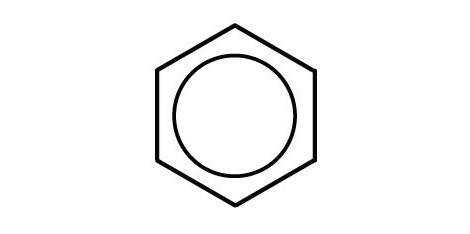
\includegraphics[scale=0.4]{benzene.jpg}
\end{figure}
\vspace{-1cm}
\tab \dashh 那是什么?\\
我说:不知道啊。 他说: 那是 benzene,6 个碳原子组成的分子。  我就那样转了系。

心里常怀疑,堂妹抛弃了我,最重要的原因会不会是因为我是\uline{中国}人? 那就是她唯一说不出口的原因吧?  因为无论我和她如何使劲的 fuck,也 fuck 不出金发碧眼的婴儿,而我和她的人种是次等的?

多年来我一直想,想她为什么不肯说话,我想靠自己的推理推出她不肯说的话。

而,居然就在这绝望之际,找到了解决的办法。 这解决办法是那么好,it is far far better than anything I have dreamt of....

\chapter{监视下的日常生活}

或者描述一下长期活在真人秀里是一种怎样的感觉。 

被堂妹和亲戚打了一顿之后,我肯定堂妹不喜欢我了,於是我可以名正言顺地开始追求新对象,想到那些\uline{美国}大学的女孩很漂亮性感,甚至咀角泛起了一丝微笑。  原本就不是很瞧得起这个身材胖胖矮矮的穷家女,失去了她又怎知不是福气?  这样想著,我走出大学宿舍到饭堂吃晚饭,在电梯内遇见两个金发的漂亮女生,她们在谈话。 \uline{美国}有些女孩谈话时语气很特别,就算她们在说些无聊琐事,也好像你们男生应份要对她们关注。 其中一个女孩语气有点夸张地说: ``I think he's really an \textit{asshole}!'' 似乎在谈论她们认识的一个男生。  但我却似乎很明显地感觉到这话是冲著我来説的,因为我堂妹不是不喜欢我,她掴我是因为我的爱是假的,而我顺势放弃了她另结新欢了。 我很卑鄙....~ 是吗?

\vignette

有次暑假从\uline{美国}回来,探望嫲嫲,她喜欢在她家开著电视机。 我听到电视剧里的一句对白。  我自己从来不看电视,完全不知道是哪齣电视剧,也不知上文下理,就只听到一个男的声音说:『唉,他们两个都这么鄙劣,真是\ds{天造地设}的一对!』  我立即觉得他们是在映射我和堂妹,心里很厌恶:「难道你们偷看我,就不鄙劣?」  然后又想: 为什么觉得他们在说我呢?  这岂不是「对号入座」?

这样的感觉几乎每天也有,只要听到或看到别人的閒言閒语或任何琐碎的事,都会联想到是在映射自己。\footnote{在精神病学中这个病徵叫 ideas of reference。} 

有时在家里自言自语,说了特别好笑的笑话,又会沾沾自喜,觉得全世界的女孩都听到了我聪明的笑话。

但当有些瘀事发生,则又会非常愤怒,因为我从来没有默许过这种监视,觉得全世界都在欺骗我,他们始终有一天要赔偿的。

\vignette

有些事情很巧合,无法解释。  刚从\uline{美国}回来,那时我仍是特别喜欢白人女人,有一天在网上看到一个\uline{欧洲}贵族的公主,她接受访问,头上戴了头箍很清纯可爱。  我想起来,实在很多年未见过女人戴头箍了,似乎这年代已经不流行。  然后我又庆幸自己能在真人秀里间接地「结识」这位\uline{欧洲}贵族,在沾沾自喜。

那时家里有个\uline{印尼}籍的傭人,她的样子也很漂亮,但可能是主仆的关系,她老是跟我作对,令我很烦厌。 奇怪的是,我在网上看到那\uline{欧洲}公主的第二天,那\uline{印}傭女孩竟又「东施效颦」地戴了头箍出现。 我那时期正和她闹得很不愉快,看到她头上的头箍,顿时产生厌恶,因为那就像是对我说:『你不喜欢我吗?那我也要破坏你和\uline{欧洲}公主的好事。』

回想起来,其实那\uline{印}傭天天换发饰,另一天她又变成 dreadlocks,所以有一天戴了头箍也不足为怪啊。

\vignette

最近有一次,认识了一个\uline{大陆}的女朋友,我告诉她我接近中年以后比较少运动了,清洁家居就是我的运动。 然后我们在家看电视,那天是愚人节,我们看到一种很奇怪的运动项目,看起来像有个机械人吸尘器,另外两个人在旁边用地拖拼命地抹地。 我越想越怒,觉得那些电视制作人利用愚人节这机会来揶揄我把清洁家居当运动。 女朋友听了后翻白眼说:『天啊... 那是``冰壶''啊...! 我以前也未听过这种运动....』

\begin{figure}
\centering
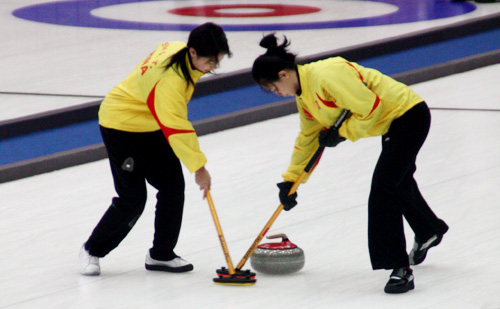
\includegraphics[scale=0.6]{curling.jpg}
\end{figure}

\chapter{爱情}

或许因为性格内向,我常常在网上的聊天室认识女性,也有不少女孩「上钓」。 有时我觉得,这些女孩独具慧眼,懂得欣赏我的见解,而且她们爱国。 但如果这真人秀不存在,那些女孩根本不谈任何条件,就会在网上免费和你做爱,甚至我是个疯汉也没问题?  我那么辛苦读书、做研究,有区别吗?!

有个\uline{香港}的大学女生,只在电话上谈了一会色情,便在当晚来我家过夜。 她见到我后有些挑剔,似乎不满意我的外表或年龄,我心里开始有些不快,又想起较早前在网上看到的AV片,那AV女孩在片中做爱做得很开心,而我觉得这些AV女优都知道我是谁,她们有时间开心地做爱,也不告诉我一声我被人偷看,让我这样被钉在十字架上很多年.... 越想越想.... 我和那女生躺在床上聊天,她问我喜不喜欢她,我就晦气地说「普通吧!」 然后第二天早上她说她要走了,我没有挽留。

她走后,我发觉自己很喜欢她,哭得很悲恸,我搞不清为什么她要走,也搞不清是不是因为这妄想病令我说了不该说的话。 几天后我到她读的大学图书馆还书,看见路上的女生有她的影子,路上行人的眼睛红了好像想哭,好像举世都为我而哭了。

临别前她说: 我也希望你快乐。

\vignette

我发觉我在网上做爱时,是用没有被监视的那边脑子,而如果一面想著被人监视的话,根本无法做爱。

据说有些野生动物,牠们只会在野外交配,被人类困住之后就不会交配,所以只有例如牛、马、狗等种类能被人类驯养。

但可惜我有时会用另一边脑袋和女孩说话,可能把她们吓跑了....

而且我也察觉到,自己的脸两边越来越不对称,一只眼比较大,眼眉较高,看上去很开心和善良,另一只眼较小,眼眉较低,看上去很凶,像杀人犯。\footnote{我研究过神经科学,当然知道左右脑的关系是很复杂的,我只是用左右脑比喻我的精神分裂。 据说有些人的眼睛不对称,是因为一边脑控制面部表情较强,久而久之,造成两边不一样。}

\begin{figure}[H]
\centering
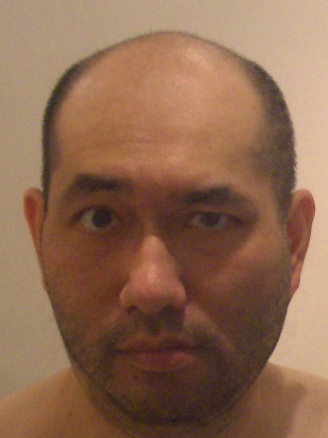
\includegraphics[scale=0.6]{2015June.jpg}
\end{figure}

\todo

曾经很长的时间我一直觉得这世界的人的吸引力可以排成数学上的序列,例如: \\
\tab \tab \tab A 拒绝了 B .... B 拒绝了 C .... C 拒绝了 D .... 
\begin{center}
\begin{tikzcd}%[row sep=large]
\mbox{A} & \mbox{B} \arrow[l, "\heartsuit" red]
& \mbox{C} \arrow[l, "\heartsuit" red] 
& \mbox{D ....} \arrow[l, "\heartsuit" red]
\end{tikzcd}
\end{center}
那么 D 的吸引力必定远低於 A; D 会喜欢 A,但 A 不可能会喜欢 D。

换成我自己知道的实例:
\begin{center}
\begin{tikzcd}[row sep=large]
\mbox{初恋女友} \arrow[r, "\heartsuit" red]
& \mbox{我} \arrow[d, "\heartsuit" red] \\
\mbox{Jimmo}  \arrow[u, "\heartsuit" red]
& \mbox{堂妹} \arrow[l, dashed, "\scalebox{0.8}{?}" red]
\end{tikzcd}
\end{center}
我因为堂妹抛弃了初恋女友,而她在外国旅行时结识了一个 Jimmo,他是个艺术设计师,他很喜欢她。

\chapter{妈妈}

未能去\uline{纽约}找堂妹前,我在\uline{香港}想念她,又没有通讯。 那 5 年间我的生活极度抑郁 (depressed),又怪我父母不准我见她 (但其实她也不会想见我)。 我在房内不停写「讨厌」两字,有一天我妈居然在我的涂鸦上写着「何厌之有?」 那更使我讨厌到无以复加。 我很想说:『妈,那就是你呀!』 但那样的话实在难以启齿。 我还未解释: 我自幼便觉得我妈畸恋我,感觉像那电影《Fatal attraction》(但我其实未看过它)。 过了几天,我终於忍不住对她破口大骂,大意是指她不守妇道、我是我、她是她、我不是她占有的、等等。 听我爸说,她那天晚上哭到不能止哭。

自幼,我爸不能驯服我妈,又对我妒忌,因琐事借故拿我出气。 至少我相信是这样。 而我爸做错了什么? 难道他这生有出卖过任何人? .... huh?

但我妈的思想大概没有那么深,她只是说:『这世上人们互相利用,谁都是这样。』 我也不认为她讲得不正确,只是有些浪漫的人不会说得那么露骨,而我喜欢用客观的科学去分析一切。

有一次我们在外国旅行,和一些远亲吃饭,亲戚中有个丧了夫的寡妇,而我妈和她说笑,说什么『老公早点死掉还更开心。』 而我爸坐在旁若无其事地吃饭、付钱。 从小到大,我看见母亲都是这种态度。

有时期常叫我父母离婚,因觉得我爸受蒙骗,是一颗终会瞒不住的计时炸弹。 但有一次争辩中他冲口而说:「我也有个情妇,她也叫 Anna (我妈叫 Anna),你是不是想见见?」 我顿时啼笑皆非,这实在太正常了。

在\uline{纽约},我在伯娘家的厨房偷看堂妹的笔记,发现她写了些少女情怀的诗,使我像着了魔那样好奇。 晚上她放学回来, 抢了笔记本然后对我破口大骂。 那天晚上我回到大学宿舍,在床上哭了一晚,一面哭一面自慰了很多次,这生人都未试过那样。

后来,我想忘了她,继续\uline{亨利8世}的计划,但我大概不会再那么爱一个女人了。

而我又想,那些偷看我的人,也应该受到同样的教训....~ 如果真有其事的话。

\chapter{打阿妈事件}

入精神病院的直接原因,是因为打阿妈。 我很讨厌妈妈买东西给我,例如衣物或日常用品,而她几乎从不买东西给弟弟。 可能是因为弟弟很喜欢高品味的东西,而我比较不修边幅,我这辈子通常都是穿著别人买给我的衣服。 其实是因为我注重环保,而明白到物理学上的物质和能量守恒,令我经常把世界看成是近乎零和游戏那样; 这对於不懂科学的妈妈和弟弟可能很难理解。 好不容易才把一件讨厌的衣服穿烂了,妈妈旋即买一件新的回来。 又,因为我穿那些老土衣服穿厌了,开始把衣服反转来穿,而妈妈竟然买了一件款式是露出线缝在外的 T 恤给我,尺码又紧又不舒服。 还有一次,我看到外国人的笑话,说「如果你....,你就是\uline{中国}人」, 其中一项是「你把牙膏用到像纸一样扁 。」 我觉得很好笑,於是故意把牙膏压得扁扁的。 谁知妈妈买了一个用卷轴挤压牙膏的工具,还把它卷在我的牙膏上,摆在洗脸台前。 世上有很多人不够衣服和日用品,而我眼白白看着这些物品浪费,简直是折磨。 我已经跟她解释了无数次\footnote{虽然在数学上是有限次},包括那环保理论。

我发觉她根本不是关心我,而是在赌气,因为不想我追到漂亮又聪明的洋妞而变得性格乖戾。 有一次我甚至\uline{中英}文粗口并用来骂她买东西给我,她说:「噢,你讲粗口,我不跟你谈了....」 然后她又承诺不再买东西给我。

我那时已经是成人,2009 年,38 岁,脸上长了第一根白须。 和家人同住实在太多磨擦,所以妈妈决定给我买间房子。 本来我想买便宜的,为了保存资金作人工智能的创业用途,但妈妈结果买了 3 倍贵的房子,也不用徵询我同意(尽管这投资现在看来是不错的)。 我在看楼的时候发脾气骂她,而我爸说:「我就想到他一定会骂 …」 后来我们去买家俬,我自己选了一张像钢琴形状的黑色桌子,而我从来不懂弹琴,所以那天心情特好。 我用轻松的语调警告我妈「不用给我的房子添东西啊,我自己会买!」 这样叮嘱了 3-4 次。

\tab \dashh 热水壶呢? 你一定要煲热水的。\\
\tab 我说:不要,我想自己选,我也喜欢购物。\\
\tab \dashh 小型的电焗炉。\\
\tab \dashh 不要。\\
我还向她解释了为什么不用焗炉,因为高温焗东西会产生 AGE (advanced glycation end-products),加速老化。 姑勿论这健康理论正不正确,每个人有权管理自己的健康的,各位读者有没有异议?

记得是一天后(顶多是两天),我下楼看到妈妈已经把我的物品包扎好了准备搬家。 妈妈在楼上,爸爸好像有第六感去了郊外散步或游泳。 我心跳加速,用刀剖开纸皮箱,果然看到那两件东西。

回想起来,一个人买礼物送给我,就算她的动机多么可鄙,我也没有权打她。 事发前我们已经找过社工来排解纷争,那时妈妈辩解说:「母亲爱儿子,有什么不妥?」、「我不爱你爸爱谁?」

其实那也是我想问的: 「妳口口声声说不爱我爸,那妳不爱他爱谁?」

我觉得实情是她后悔以前畸恋我,现在和我斗气。

我拿起焗炉跑上楼,把它狠狠地摔在她房间的墙上,然后掴了她一下,又拿沙发椅子摔向她,并要她跪下来道歉。 之后我知道脾气暴躁的爸爸回来后必会导致命案,所以我拿了厨房的菜刀,反锁在自己睡房,用床诸塞门口,然后报警。

那些警员是父亲以前的同事,他们都想大事化小。 众人都已归於平静,但我爸坚持要我到医院检查精神有没有问题。 精神科医生要我住院一晚以便观察。 他们和我谈的时候,我天真地想,不如借此机会请教他们我的 paranoia 问题 —— 而的确,我很需要人帮助。 但我得到的「帮助」完全不是那么回事....

自幼,不知是不是母亲的间接暗示,我常喜欢模仿疯癫的行径,母亲大概觉得那是有才华的表现,我也自觉很有意思。 我的同学朋友也知道。 想不到现在真的变了「疯子」,但我惊觉那不是闹着玩的,就像老鼠怕老鼠夹,那疯人院对我而言真的是 booby trap。

为了逃离疯人院,我迫於无奈,在探病时抓着妈妈的手说:「妈,我很疼你.... 快救我出来。」 那就像「芝麻开门」那样有效。

出院后我和妈多了谈话,因为要定期覆诊,要「表现良好」。 我搬进新屋,但不久之后妈妈送的礼物又再像恶梦般回来。 先是 4 只凉衣架 —— 我其实真的不够凉衣架用,但看到那些凉衣架真有欲哭无泪的感觉。 终有一天,我会追到女朋友,逃离她的魔掌,绝不能被 4 只凉衣架搞到性无能。 我向她解释:「新闻说有个痴情男子在餐厅铺满玫瑰向女子求婚,但也被拒绝了。 若他每天送玫瑰,送十年,天天浪费时间和资源,那女孩也不想要,对社会也没贡献,这样做人有什么意思? 我也接受了堂妹不喜欢我的事实…… 我现在连她在地球哪一洲也不知道。」 我妈回答说:「不是的,你不知而已。」 Huh? 难道我堂妹还喜欢我? 已经想了十几年,以为抛却在背后了,究竟还要想多久才有结论?

究竟我妈明知我不想要却坚持要送东西给我的动机是什么? 如果她真的为我好,应不会这样吧? 有时甚至怀疑她老人痴呆症,但她又否认。

我妈不喜欢吃太甜和冻的东西,我想最好每次见面在 7-11 买杯思乐冰 (Slurpee) 给她。 那种东西在整个冬季有没有人按一下都成问题,但又见它不断在搅拌。

在\uline{美国}时,有一次在堂妹家的后门等她回家,等到深夜,见她的车子开进来,被车头灯照得睁不开眼。 我可怜兮兮地望着她,想博一點同情分。 等她泊车,谁知她是在急速掉头,想避开我; 在那很窄的空间,她驾车技巧的纯熟令人诧异。 人们常说女人驾车「姐手姐脚」,但她们发怒的时候比赛车手还凶。

我明白到,不想要的爱,是会令人感到极度烦厌的。 有次我和堂妹在她家门口纠缠之际,我看见她的眼里也有泪光,但那跟我的眼泪是有着 180$\degree$ 相反的意思: 她觉得我可怜,但又不喜欢我,但又被我的苦苦纠缠弄得很痛苦。 为什么被痴缠的人总有那么强的欲望去让痴缠者死心,好像不那样做不行? 但每个月收些不想要的礼物,又真的会逼到人发疯。

我偶然看过 Tom Cruise 到\uline{中国}做宣传,那些年青的\uline{中国}女子,多得像人海那样,她们伸长了手臂在召唤偶像,泪流满面、歇斯底里地喊着。 照上面的理论,那傢伙肯定定变性无能了(因为有那么多单恋他的女人)? 但后来又想到,Tom Cruise 是自愿当明星的,那是双方自愿 (consensual) 的偶像-影迷关系。 有天我也想在台上引吭高歌,听台下万千观众的欢呼....

妈喜欢看书和看电影,《红楼梦》、《罪与罚》、《飘》那些书她都从头到尾看过,又怎会是那么笨的人? 她最喜欢的小说是 Jack London 的《海狼》。

在《知乎》网站上看到人们评论一则新闻,说有个无经验的大学小伙子,在女生宿舍楼下求爱,用洋烛摆了 I LOVE YOU 的字样,但那不领情的女生走下来用水盆把洋烛泼熄了,还用盘子扣在男生头上。  类似这样求爱不遂的事件时有发生,我看人们在网上的评论,察觉到很多人是非不分,评论别人时什么离谱的话也说得出来。 如果说那男的做错了,他做错了什么?  如果他纯粹缺乏经验,那女生有什么权打他呢?  这件事就和我打送礼物给我的妈妈一样,只不过男女角色互换了。  但我觉得我妈明知我不喜欢她送礼物却故意送给我,是在挑釁。  而那男生也有可能明知女的已经婉拒了他,却仍然装蒜在跟她斗缠。

%印象中我接触的很多西人,评论事件时态度认真,像写哲学论文,但回想起来他们的混帐言论也很多。 

\chapter{爸爸}

不想将这本书写得太长,只想借一件小事描述一下我爸这个人。

他是一个脾气很差,但有急智,做事很注重纪律和效率,但知识上不是很精深的人。  他喜欢读历史书,厚厚的《\uline{邱吉尔}传》他看完了,还有一套《\uline{中国}历史》,全套像手臂那么厚。  但他看完书从来不会谈论,不像我妈那边有个满腹经伦的舅父,常常高谈阔论。 他喜欢爬山,我们亲戚笑他临睡前的 light reading 是地图。

自从我打了阿妈之后,弟弟发怒~不睬我。 这令我觉得很遗憾,因为我在这世界上几乎没有朋友,现在连弟弟也不睬我。 后来有一晚中秋节,妈妈说约了嫲嫲到酒家吃饭,弟弟也会来。  我心情很好,因为已经一年多没有见他。  那天天气炎热,我步行到酒家已经流了很多汗,很不舒服。 到场时我问: 咦? 弟弟呢? 妈说: 他 .... 临时说不来了。 我顿时很失望,还用咀「啫」了一声。  总觉得我妈时常想见我,就编各种借口引我来,其实她一早就知弟弟不会出现。 我心情烦躁,叫嫲嫲的傭人(她陪我们来吃饭)给我找一只杯斟水。 找到杯子后,我爸也拿他的杯子端到我面前:「\uline{景贤},帮我斟点茶。」

其实我自从\uline{美国}回来后,对於所有「主/仆」关系都很反感,尽量不想摆架子,但那天却因为心情烦躁,很自然而然地叫了女傭做事。  而我爸居然在那么短时间内「以牙还牙」,反应之快令人咋舌。

对了..... 想起来了:~ 我爸无法奴驾我妈,却常常为了争风呷醋而找岔折磨我。  我妈明知爸爸在拿我出气,却经年累月的装作看不见。  那就是我肯定不会喜欢妈妈的原因。

\string{ 蛋糕 with shit \string}

\chapter{精神病院}

在正式关进精神病院的时候,有男护士要我签字同意治疗,我问他说如果不同意会怎样? 他说就算不同意也会强迫入院,所以没有分别。 后来我出院后到精神病人福利团体那里了解,其实我是有权不接受治疗的。 那些精神科医生很想关病人入院,因为不这样的话他们没有生意,他们收入的来源其中一部分可能是由\uline{美国}的药厂赞助的。 精神科药物为\uline{美国}经济带来每年很多亿元的收入。 他们找个低级的护士迫我签字,那样便毋须负责任。

医院里光怪陆离,像动物园,如果不是没有自由,那会是个很有趣的地方。 有个来自\uline{大陆}的年青人,他说「我妈不知给我喝了些什么汤,喝后会使周围的人知道我在想什么。」 我说话开导了他一下,但那时我也自身难保。 其实他的病和我的病一样,但我受过科学的教育,不会迷信,我的病以不违反科学的形式呈现出来。 他整天听家人给他的收音机,学\uline{广东}话。 那令我想起,\uline{香港}人普遍歧视\uline{大陆}人,就像\uline{美国}很多人歧视我们华人一样。 我和他都感受到周围的人的敌意,产生了逼害妄想。

病友中还包括:
\begin{itemize}
\item 一个因前妻外遇而自杀过的中年人,要吃开心药。 他很健谈,常对我们讲历史;
\item 另一个因妻子不忠而拿了菜刀和她吵架的人;
\item 一个读数学的大学毕业生,他幻听的声音常叫他做一些不明所以的事,例如丢掉某些东西;
\item 一个中学高材生,用刀割过自己的手腕,拉起袖子让我看很多条刀痕。 他说他当时像神志不清那样,不知为什么那样做。 我和他下棋,输了给他。 我向他解释神经末梢的原理(neuron、axon、dendrite、synapse 那些),建议他不要吃药,第二天他就不见了,不知是回家还是调到另一病房;
\item 一个在便利店偷东西的人,他说他自己也不知道为什么偷了几本杂志。 吃了药的他手震得很厉害;
\item 还有几个是「长期住客」,据说他们被困在细小的病房里有很多年之久。 我们病房大约两间中学课室那么大的地方,这样被长期监禁着,是很不人道的;
\item 一个在晚上会叫你「早晨」的人,但他其实也像正常人,只是很爱开玩笑;
\item 还有一个不会说话,样子像怪兽、叫声也像怪兽的怪物。 他有没有受医护人员虐待都很难说。
\end{itemize}

看过 YouTube 上外国女孩把自己在精神病院的片段登上去,我在想:怎么她们那地方像 Hotel California,而我们这里像 Iron Maiden?

覆诊的时候见过一个年青人,面色苍白,手震得很厉害,像那些心脏衰竭的老人。 那是很典型的药物反应。 我心想,他被药物弄成这样,必早死,就算将来减少剂量,他的寿命也会被弄短好几年。 这些医生简直是在慢性杀人....

如果明白那些药的作用,根本没有人会肯吃。 \uline{美国}的药厂隐瞒事实,把「毒药」输送到\uline{亚洲},而\uline{亚洲}的行政人员对他们唯命是从,毒害了无数无辜的人\footnote{虽然在数学上是有限的}。 然而,\uline{美国}或西方的没落,其规模之大可能还远远超过这样。

和那中学生下棋的时候,有个男护士走过来,看了几秒便对我说:「你在两步后会有危机。」 我看不出来,甚至在他告诉我以后,我还要下两步棋,然后才发现对方的马后炮。 据说\uline{孙中山}下棋也不高明,爱急攻,但忽略防守。 但奇怪的是我下国际象棋时认真很多,虽不算是 master,但也算攻守兼备而且比较「靠谱」。 我有个理论: 在中学时那些喜欢国际象棋的同学,比较有国际视野,而喜欢\uline{中国}象棋的人会倾向留在\uline{香港}或\uline{中国}发展。

\chapter{发病的原因}
\label{cause-of-illness}

1996 年我初到\uline{美国},心境像\uline{尼采}所说的『这杯子将再度变空』,我要虚心学习、要青出於蓝。 我对\uline{美国}人没有恶意,我要胸无城府那样接待他们,而且要为\uline{中国}人争光、不要失礼。

很快地,我发觉我无论做什么,都好像变了\uline{美国}人的笑柄。 我写了一封情信给堂妹,信封上画了我抱著她的画面,那幅画抄袭\uline{日本}恐怖漫画的美女,她的头发像\uline{波斯湾}里漆黑的石油涌进大海\footnote{这个比喻是一个\uline{美国}女作家的,忘了出处}。 内容大意说: 我来了,在 Long Island 的这间大学,我很挂念妳。 但她见到我后似乎非常厌恶,似乎我在她身旁很失礼她。

我穿的衣服、行为举止,都和\uline{美国}人格格不入,而且年龄比普通学生大一点,觉得自己在课室里很惹人注意。 而且很奇怪地,那些\uline{美国}女生不断对我抛媚眼,她们 come-on 的大胆程度,即使我思想算很开放,也令我很惊讶。

我逐渐留意到一些巧合的事,例如我在宿舍房间内做的事,很奇怪地变成了教授开玩笑的话题。 於是我怀疑有些学生在故意恶作剧搞我,因为\uline{美国}大学常有恶搞新生的事件,而这传统在\uline{香港}没有那么极端。

当我开始有被偷窥的想法之后,我做了一件(我自己觉得是)很惊人的事,就是我「将计就计」地把自己的私隐公开出去,目的是要向全世界揭发我认为是欺骗人的事。  例如我觉得我堂妹在骗我感情,我妈欺骗我爸感情,还有\uline{美国}的虚伪,他们假装和我开玩笑其实是想整我,因为他们知道我会是帝国的终结者,我的成就终有一天会盖过他们。 那是真的: 我真的有那样的抱负。

我在\uline{美国}写电邮给在\uline{香港}的前度女友,和她报告我在\uline{美国}的所见所闻,有时也哭诉堂妹如何令我心碎(我就是因为堂妹所以和前度分了手)。  她没有到过\uline{美国},我说的故事令她很感兴趣。  但我在写给她的电邮里,故意暴露很多真实的事和心底的话,而且尽量写得诚实,因为我知道我的偷窥者们一定会看得津津有味,这种真人的「演出」比所有电视那些经过彩排的假故事一定更吸引。  而当他们将我的趣事一传十、十传百那样传开去,最后帝国的谎言就会像「国王的新衣」那样人尽皆知。

这个计划似乎很完美,可惜有个漏洞: 就是我自己也无法肯定究竟有没有人在偷窥我。 当我开始想验证的时候,我发觉这件事简直不可思议地\ds{无法验证}。  所有巧合的事,都可以解释成真人秀的存在,也可以解释成巧合。

有些逼害妄想症的男人老是怀疑自己的妻子红杏出墙,即使妻子很忠贞也是如此。 但这究竟算不算是一种病? 当然,如果妳就是妻子,妳当然知道自己有没有和别人睡,但妳又怎能假设正在外面上班的丈夫知道妳私下做什么?  如果他不知道,他就有怀疑的理由,这不是很科学的态度吗?  而且这世上的确有很多红杏出墙的妻子,我在网上也和她们玩。

\begin{comment}
我和初恋女友常常因为我的怀疑和猜忌闹得很不快,但我一厢情愿地信我堂妹爱我,其实她早已不喜欢我,我白白等了她很多年,觉得这种专一的游戏很幼稚,浪费时间在互相猜忌。
\end{comment}

有了被人監視的想法令我在\uline{美国}每天的生活仿如人间地狱。  扭开电视,看到有科幻片叫《星际笨蛋》\footnote{Inter-galactic Idiot},我以为他们在嘲笑我。  无他,因为他们必须永远假装在开玩笑,否则便要面对老实地谈判。  我初时常常觉得\uline{美国}人的幽默很好笑,但越来越觉得他们笑里藏刀,是一种恶意地贬低别人的心理战术。

终於毕业,回到\uline{香港},我在行李箱内放了我以前写给前度女友的所有电邮(每次写完比较长的电邮就用学校的打印机印出来),那是重要的记忆,作为日后参考之用。 我在\uline{香港}待了约一年后,突然有一天怎样找也找不到那些信件。 问我妈,她的表情天真得像个 13 岁小女孩,她说:『噢!我丢掉了。』

她不是蠢,而是占有欲很强,把儿子当做一件附属的东西。  这不是她唯一一次想毁掉我的记忆; 第二次是在精神病院里,如果我不机警,那些精神药已经令我变了傻子。

如果不是写这篇自传,我差点把这件事忘了。  现在我很愤怒,我不是想打阿妈; 我简直想杀了她。 

我看过一本\uline{英国}女人写的自传,她少女时被父亲性侵,他还约朋友到家里把她按在床上轮奸。 后来她离家出走,找到了肯爱护她的男人。 我自己也是个好色男人,有时喜欢扮 daddy 和女孩玩幻想的轮奸游戏,看到她这样厌恶父亲,不免感到有点「没趣」,但当然她是对的。  也听说过有些父亲和女儿变成了情人关系,我觉得只要是双方自愿的,那样也没有什么不妥。

不时看到很多歌颂母爱的电影,令我非常厌恶,我觉得他们故意站在我妈那边。 我妈假装她爱我,其实我要揭发的人,其中之一就是她。  她假装骗我是为了我好,因为如果不骗我的话,\uline{美国}那边会派人杀了我。 但其实\uline{美国}政府已经处於劣势,他们想为所欲为也有制肘。 我妈和某些\uline{香港}人、\uline{中国}人,他们妒忌我计划的成功,故意将\uline{美国}说成很强大,作为他们出卖\uline{中国}人的借口,继续骗我。

\chapter{和堂妹相似的人}

最近事情又有了新发展:  接近 100 岁的嫲嫲生日,我们一班亲戚在酒家吃饭。  席间, 冷不防表姊提起要打长途电话给堂妹们让她们道贺。  我听错了以为她们又来了\uline{香港}探亲,要上来酒家,突然间我的面容很可怕地扭曲起来,像遇到多年不见的仇人,过了整整 3 秒才 regained composure。 我觉得表姐们一定看见了,而她们都知道我和堂妹的瓜葛。  我也很奇怪,明明觉得自己想通了,现在已经很释怀,和其他女人玩得很开心,但原来心理上还是留下了很可怕的阴影。

表姊们传递手机上的照片给我看,我看不到堂妹,但看见她新近结婚生下来的BB。 那婴儿房的布置,整间房间都铺满了老虎的毛毛玩具,俗不可耐。 我暗付:『好彩当年追不到她。』  过后又想起: 她还是没变,还是像老虎那样凶,动不动就想打人。

又过了一两年,在网上居然发现了她的 Facebook,我看到她的老公是个白人,样子端庄,还算给人好感吧。 可是我看着他们来\uline{香港}旅行的照片,怎样也感觉不到一丝快乐。 我身边的新女友说:\\
\tab \dashh 他们看上去很快乐啊 \\
\tab 我说: 是吗?

在 Facebook 上 add 她,但她没有回覆。

过了不久又传来她儿子的相片: 那小孩子一头金发,身上完全看不到一丁点\uline{中国}人的特徵。 她应该感到很欣慰了吧?

听亲戚们说,她很喜欢游泳、潜水。  我怀疑她还记不记得起\uline{布殊}喜欢打高尔夫球....?

回想起来,我堂妹很不喜欢说话,可能是因为我们言语不通,她说的\uline{中}文很有限,而我又很爱面子地不肯在她面前说\uline{英}语。 在\uline{纽约}那段日子,我能够记得起她说的话,就只有一些单字,她就像个白痴那样只会说单字,但又好像想用那些单字来迂回曲折地暗示些什么。 我们一起吃晚饭,她和我妈谈到在\uline{美国}的商店买货品,凭单据可以无条件退钱或换货品(\uline{香港}人会觉得很惊讶)。 她突然煞有介事地说:『\ds{交换}嗱!』用的发音有点偏差的\uline{广东}话。 在送我往机场的路上,她指著机场附近的人群说:『噢,有那么多\ds{中国人}!』  我堂妹真是全球说话最拐弯抹角的人。

她姊姊说话比较直接 \\
\tab \dashh 你觉得我妹妹在 egg you on, right? \\
\tab \dashh 你是不是觉得我们在\ds{出卖}你呀? \\
\tab 我被气得对她姊姊破口大骂: 听著! 我永远也不会原谅妳们的! \\
\tab 但她姊姊狰狞地说: 噢\textasciitilde\textasciitilde~~ 我们很害怕呀\textasciitilde\textasciitilde ~!

其后我常常思量堂妹说的「交换」的意思。 我在网上结识很多白人女孩,处处在她们中间寻找堂妹的影子,但始终没有人和她太相似。 直到我放弃了找白人女友,我开始约会一个\uline{中国大陆}的女孩。 我已经忘记了「交换」。

\vignette

那\uline{大陆}女孩身材有点矮矮胖胖的,和我堂妹一样(也和我妈一样),但我初时没有联想起来。

我们在散步,地上有一块「小心地滑」的牌,她看了后侧著身轻轻地滑了几下,说是『小心地 ~滑』。 那姿势令我想起堂妹跳蹦蹦时也是这个模样。

在餐厅她点了红豆冰,她说她喜欢红豆,但不喜欢冰冻的东西。  我突然记起: 我妈也喜欢红豆,她也不喜欢冰冻的东西!

我和她的关系急转直下,差不多为每件小事都意见不合。 她做错事从来不\ds{道歉},而且觉得自己永远是对的。 她说话很特别,常常自相矛盾,在5分钟内可以 $A \wedge \overline{A}$。  我记得14岁时的堂妹也是这样,令我感觉奇特,但我已记不起她当时说的什么话题。  堂妹14岁时常常无情地批评我,我那时觉得她身体是个小女孩,心灵却是1000岁的精灵。  现在面对这个「堂妹2号」,她虽然已经27岁了,我觉得她竟蠢得像1000年未用过脑。% 又想起我妈,我觉得她简直生来就是老人痴呆症的。

我很喜欢\uline{村上春树}的比喻:「一切都像描图纸那样错开了....」

好几次看到她在哭,因为我不喜欢她了。  我的心隐约感受到记忆中很久以前的痛,因为她就是以前的我。 我想对待她好一点,尽量做得和堂妹对待我不同一点,因为我要证明堂妹那样对我是错的。 我很耐心地将一切解释给她听,甚至这份自传也是写给她看的\footnote{或者说想写给我将来会认识的所有女孩},但她说她不像我堂妹(她似乎无论我说什么她也持相反意见)。 我很愤怒,觉得她不可理喻,语言好像对她失去了效用。

我说: 我可以教妳怎样变聪明点,但即使妳改变了,我也不会喜欢妳,正如一个雕塑家不会爱上自己雕的石像,我也不能将妳打扮得性感漂亮 ~然后爱上妳,因为那就不是「爱」而是「自慰」。

我说: 对不起,但我也希望妳快乐。 (就像那一夜情女孩对我说的那样。)

我刻意地开导她,令她不再犯我当年犯的错误,但她就像一个考全A的女生,将所有功课交齐: 我以前对堂妹所做的每一件卑劣的事,她像有只第三眼那样回赠给我,真令我感到「天网恢恢,疏而不漏」。 有一次我在\uline{纽约}的唐人街买了一盒人参给堂妹她们, 因为我觉得人参是\uline{中国}特产,可以令堂妹想起我们本是同根生,而且我记得妈妈小时候对我说,有些人参生长得像人形,濒死的病人吃了也可以起死回生,令我觉得很神秘。 我送了给她们,她姊姊对我说:『谢谢你啊,这人参含有 stimulant,吃了感觉精神很多。』  其实她婉委的意思是说: 不要迷信人参是神奇的药,它只是含有一些化学成份。 我自小喜欢科学,讨厌迷信,但我糊里糊涂地选择了这样的礼物给她们,目的是想说: 为甚么嫌弃我落后呢,妳们陪我一起落后不好吗? 后来我转了读生物化学,整个人彻头彻尾地科学化了,那次「人参事件」为迷信的棺材钉上了最后一口钉。

其实所有「初到贵境」的\uline{美国}华侨,都要经历过这些学习,每年成千上万的新移民经历著同样的事....

\vignette

教她写程式,因为我想要一个懂得人工智能的女朋友帮助我,但她碰到一些难题就发脾气。 例如我教她 nested loops:\footnote{巢套迴路,但我当时还未想到用这个 X loves Y 的例子。}\\
\code{
\tab for i in ["john", "pete", "paul"] \\[-6pt]
\tab \tab for j in ["mary", "ann", "jane"] \\[-6pt]
\tab \tab \tab print i, "loves", j } \\[5pt]
她弄不懂却发脾气,甚至我觉得每次在就快到解释明白的关头,她就故意发脾气,让进度拖慢到零。 有时我怀疑她是不是 CIA 派来的特务,目的是拖垮我的 AI 研究?

发脾气之后,她躺在床上看 iPad,我以为她悔改了,在上网学习,问她 \\
\tab \dashh 妳在看甚么? \\
\tab \dashh 在看\uline{张爱玲}的生平

\uline{张爱玲}和\uline{胡兰成}恋爱,而\uline{胡兰成}曾经因为亲\uline{日}而被后世认为是\uline{汉}奸。

我很失望: 区区一个 nested loop,妳就立即想到做\uline{汉}奸,太可耻了吧?

我对\uline{张爱玲}认识不多,但因为这件事而对她也产生了不好的印象。 据说她的小说著重描写小人物的情情塌塌,有批评者说她难登大雅之堂。

我觉得\uline{张爱玲}的样子不好看,像只蛤拐。 \uline{大陆}女友的正面虽然很漂亮,但侧面也很像蛤拐!
\begin{figure}[H]
\centering
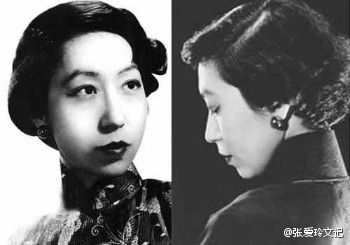
\includegraphics[scale=0.75]{Eileen-Chang.jpg}
\caption*{\uline{张爱玲}}
\end{figure}

\uline{大陆}女友对\uline{日本}特别怀有仇恨,这在\uline{中国}人当中也算常见。 而我特别不喜欢\uline{美国},对\uline{日本}却比较有好感。  很多\uline{中国}人念念不忘\uline{南京}大屠杀,但却忽略了\uline{日本}被原子弹炸的惩罚。 这世界上很多人抱著类似这种低级的历史观,难怪国际间纷争不断。

其实我觉得像\uline{汪精卫}、\uline{胡兰成}、\uline{蒋介石}那样的人,他们对\uline{日本}妥协并不算万恶不赦,或者可以说他们看清了现实,选择了折衷的办法。 \uline{汪精卫}在\uline{申亥}革命中几乎为国捐躯了,他不会是不爱国的人吧?

\vignette

\tab 我没有嫌妳是\uline{大陆}人 \\
\tab 我也没有嫌妳家境穷 \\
\tab 我也没有嫌妳腿不够长 ~~侧面像蛤拐 \\
\tab 但我不能接受妳说话 $A \wedge \overline{A}$ ~~而且永不认错

她跪在地上,很生气地说:「我现在跪著认错了!!你满意了吧!?」 

但我说: 妳不是真的认错,妳没有改!!  她想跑到厕所避开我,我追著她进去,问她 \\
\tab \dashh 妳究竟改不改!? \\
\tab \dashh 不!! 我会改! 但不会是为\ds{你}而改!

我真的觉得呼吸困难。 她、妈妈、堂妹 ~简直是三胞胎。 我不想打她,因为我要做得比堂妹更好。  但她的荒谬行径和说话,好几次令我想狠狠地掴她、想用尽全力地用腿将她撑开,让她飞撞到床外的电视机上。  我最终没有打她,但已经愤怒得身体在发抖。  我又想起来了.... 『有些女人就是喜欢将男人激到暴跳如雷....』

我仿佛听见她在讥笑我 \\
\tab \dashh 你现在终於尝到身材矮小,腿又变不长的滋味了? \\
会不会天生有缺憾的人,将他们的痛苦像毒瘤那样移植到别人身上?  但我又想: 她应该不会那么阴险吧,怪错了她?  堂妹也常常骂我\ds{下流},但有时我也莫名其妙,自己不算那么卑劣吧?

有缺陷的人也可以是好人,但不幸的人没有权加害那些较幸福的人。 如果是那样的话,\uline{中国}有那么多样子长得丑的人,岂不是要变世界强国了?

但\uline{中国}真的正在变世界强国啊....

\vignette

她进了她的房,关上门。  我在屋子里心绪不宁,打开雪柜,看见她吃剩的泡菜伴饭。

我想到她可能是个阴险的人,可能会因为妒忌而在我睡觉时用剪刀刺死我,所以我也反锁上门,才敢躺在床上睡。

但又想起在\uline{大陆}很多贫苦地方,很多人吃不到肉.... 在睡房里哭了。



「交换」是假的.... 她两次都不喜欢我....

但我警惕自己,她们是两个不同的人,不应该混淆了,但感觉上真的像被同一个人抛弃了两次。

我写了这条公式:
\begin{equation}
\mbox{堂妹} : \mbox{我} = \mbox{我} : \mbox{堂妹2号}
\end{equation}
但她不赞同,她说她没有像我缠著堂妹那样缠著我。

但问题是,其实我也没有明知堂妹不喜欢我还缠著她,而是她一直令我觉得她喜欢我,所以我才缠著她(而这也是令我百思不得其解的地方)。

可能这条公式才是对的?
\begin{equation}
\mbox{堂妹} : \mbox{我} = \mbox{堂妹2号} : \mbox{我}
\end{equation}

\vignette

以前堂妹公然和我同学调情,令我受了很大震惊,因为年少的我不懂得怎样应付这种同时和几个男孩玩的「婊子」\footnote{这个字有贬义,在男女平等的今天是不应该使用的。}。 后来我想通了,觉得一个人同时爱几个人没有什么不妥,不论是男或女。

为什么 20 多岁时的我那么蠢,在堂妹走后我试图和初恋女友复合,但却发现好像有无法填平的鸿沟。 以前那初恋女友也常常亏待我,令我在大学里像只丧家狗那样跟著她。 但自从遇过堂妹后,我的女友好像被她下了降头,以前的吸引力都没有了,整天哭哭啼啼。 我想: 为什么妳就不能像以前那样呢?   但她只会哭,我跪在沙发旁帮她递纸巾,这样默默地抹鼻涕抹上一小时。 我甚至觉得很闷,但又不忍心再伤她的心。

有一次我们讨论这问题,我想到「不如妳们两个我也喜欢不就行了?」 几乎说了出口,但又不好意思讲出来,觉得那好像违反了什么道德。

有了互联网之后,我知道这东西叫 polyamory(多元爱),那就越来越习以为常。

有一次我和大陆女友逛街,我留意到女店员很可爱,之后我随便地对她说我觉得女店员很漂亮,看她有什么反应。 她过了几条街之后突然找岔发脾气,闹得在马路上当众失礼。  事后费了很多唇舌,她才肯承认是因为妒忌的缘故(其实很明显的)。  但她对我不诚实地砌词狡辩了很久,这过程令我觉得极度烦厌。

我说: 我们已经说好,大家可以有别的男女朋友;~ 我没有做错,但妳还是呷醋。

她说: 你这样要求别人承认妒忌,并不是任何\ds{人类}能够忍受的。

可能她说的是对的:  我其实也正是无法接受堂妹喜欢别人,而几乎疯了。

回想起来这一切都那么愚蠢。

我说: 现在轮到疯的是妳。  但我希望妳看了我的书之后,那略过这个疯癫的阶段。

她说: 你错了,我和你的关系不同於你和你堂妹的关系 --- 我没有像你痴缠堂妹那样缠著你。

但我觉得她又再说谎了。

\todo

她说她不会为我而改变,我

过了不久她又再来\uline{香港},我请她来我家住。 我一番好意,以为可以帮她节省住宿费(我对於旅游时的住宿等开支总是很悭俭)。

%%%%%%%%%%%%%%%

她叫我玩 2048 (一个 4x4 方格上的数字游戏),说想看我聪不聪明。 我记起堂妹 14 岁时也和我玩黑白棋,我输了给她。  这两个游戏都不需要知识,但需要计算很多(简单的)步骤,就像魔术方块。  我最怕这类游戏,而我喜欢英文串字的游戏,她却觉得很闷。

Mushroom cloud, Clark Gable.  Book dedication.

mom and dad relation.

Hanasaki cannot help me / make me happy.

Grandma's unlikable.  Anna is an island.


\begin{comment}
我本身在政治上經常批評美國,但我自己也曾在美國留學,當然美國學歷令我在香港有點高人一等,而且我爸甚至是英國殖民時期的警司,他的錢可以說是為殖民主義服務而賺的。

問題是很多香港人憎厭我(似乎是這樣),但他們自己也變成了親英美的人。 我覺得他們不能要求我先「償還」然後再反美,因為這樣我根本不能生存。 但我已經說了會為自己過去的特權給他們補償(況且當初變節的人是我爸,不是我),那麼責任似乎就是在他們身上,他們應接受我的意見。

很多人就是太挑剔,什么也不肯妥协,其实在不妥协的过程中,他们自己本身也犯错了。 必需要成熟起来的。
\end{comment}

\begin{comment}
\chapter{爸爸}

(....)
\end{comment}

\chapter{人工智能}

这是较年轻时的 Ben Goertzel:
\begin{figure}[H]
\centering
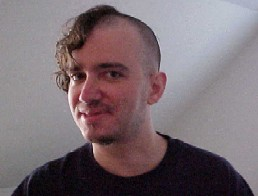
\includegraphics[scale=2.5]{benbenben.jpg}
\end{figure}

2008 年夏天,Ben 来\uline{香港}谈生意,我到机场接他,这是我们首次见面\footnote{其实在网上自 2004 年起我们已经交谈了很久}。 据说 von Neumann 首次和制造 UNIVAC 那些工程师会面,他们已经听过 von Neumann 的大名,但怀疑他名不符实,於是他们说,要看看他问的第一个问题是什么,就知道他是不是天才。  果然他劈头第一句问的就是:『电子计算机的 architecture 是什么?』\footnote{``I recall with amusement Eckert's reaction to the impending visit. He said that he could tell whether von Neumann was really a genius by his first question. If this was about the logical structure of the machine, he would believe in von Neumann, otherwise not. Of course this was von Neumann's first query.'' \dashh Goldstine, The Computer from Pascal to von Neumann [1972]}  但我去到机场时忘记了这故事,我对 Ben 说:『咦? 你的行李好少?』

Ben 问我:『你最喜欢的编程语言是哪个?』 我答是 Lisp,你呢? 他最喜欢的是 Haskell。

Ben 是 Ashkenazi Jew (那个生产最多诺贝尔奖的人种),他的某个曾曾曾祖父来自东欧(好像是 Romania),是个哲学家,研究过一些神秘主义和不是很正统的逻辑,然后几乎被世人遗忘了。 我觉得 Ben 的理论风格也有些不很正统和怪诞的倾向。  Ben 的父亲是个\uline{马克思}主义的社会学教授,他们住在\uline{巴西},Ben 年纪小时去了\uline{美国}读书,23 岁便考到 PhD(数学),而我 33 岁才勉强大学毕业。

在音乐上我比较喜欢像 Prokofiev,Philip Glass 那些新古典主义者。 我不太懂音乐,但我很喜欢和弦(harmony),觉得它很神秘,西洋音乐如果没有和声就不是西洋音乐了。 Ben 很喜欢 Buckethead (一个 virtuoso 结他手,他技巧纯熟,但在极端情况下有时像噪音)。 Ben 的理论风格也像他,而我则很注重简单和优美。

我、Ben、和 \uline{王培}教授 ~三人都不约而同地选择了 logic-based AI 作为出发点,然后都不约而同地设计了 uncertainty logic。  但我们谁都不肯用对方的 uncertainty 方法,我至今仍觉得自己的方法是最好的。 但最近我的理论方向转移,这些 uncertainty logic 的争议我已不再觉得重要。

我从 Ben 身上学到很多东西,他带我见其他生意上的合作者,但后来有些重要的会谈他不让我参与,令我觉得被出卖了。

在他开的 AI 论坛上,我提出我们所有人用电脑记录每人的贡献,然后未来 AI 赚的钱根据每人的贡献量分配,但他们不肯。

在网上互相讨论时,他们对我的态度不友善,我投诉过也没有改善。  AI 吸引很多有野心的人,但他们很多时表现得像不成熟的小孩子。  例如有次我认识一个\uline{欧洲}的新朋友,打算招徕他参加我的计划,但他却说:``I will be your worst enemy,'' 而其实我想和他交朋友啊!

初时,我企图引用反歧视的法例,例如 equal opportunity employment,逼他们接受我,但他们说那并不是所有公司都一定要遵从的法律,而是自愿执行的。 他们的不友善已经很明显,但我拿他们没有办法。

我那时很渴望有朋友和合作者(现在也是),所以我忍气吞声,没有和他们翻脸。 有个 Abram Demski 比我年轻很多,但他的数学尤其是机率和数理逻辑方面很强,我也要向他学习。 我和他还有几个朋友几乎天天讨论和合作,但后来我逼 Abram 出面和我同一阵线反对 racism,但他不认为有任何 racist 的现象。 他请我为他写报读研究院的推荐信(因为我用过少量金钱聘他做事),但我威胁他如果不反对 racism 的话我就会在信中反映。 他被我这样威胁很反感,取消了合作。 我以大局为重,说了一些道歉的话,算是勉强挽救了我们朋友的关系,但其实我对他很失望。

\begin{figure}[H]
\centering
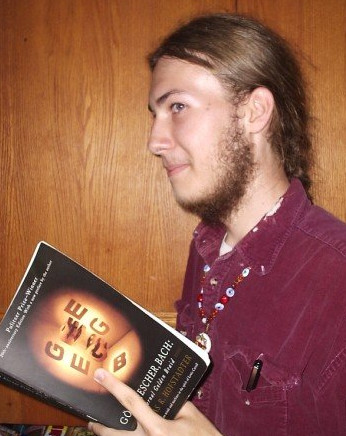
\includegraphics[scale=0.4]{AbramDemski.jpg}
\caption*{Abram Demski}
\end{figure}

\vignette

也可能是我经验不足,见到任何人有错失,便直接批评,令很多人憎恶我。  

AI 是很美妙的科技,可能是人类历史上最神奇的,我深信它能为人类带来长生不老。 而我自己很怕死,甚至是病态地怕死,我一定要通过这技术才能达成愿望。 而那些人为了好大喜功,表现得很自私,令我对白人的敬畏之心荡然无存。

但我也必需说,像 Ben 和 Abram 他们,的确很无私地和我分享过很多知识。

我想 Ben 算是个很 charismatic 的人,经常能说服很多人给他投资。 甚至\uline{香港}的首富\uline{李泽楷},他的一个助手也曾给 Ben 的 AI 投资 US\$5M。  这令我很惊讶,因为\uline{香港}人出了名不关心高科技(那时是 dot-com 时期)。 他的人脉极广,他到过\uline{日本}、\uline{韩国}、\uline{大陆}、\uline{美加}、\uline{英国}、\uline{欧洲}、\uline{澳洲}、\uline{南美}、\uline{非洲}等地,在这些地方发掘 AI 的人材和投资者。

我的数学不够专业,常被他们瞧不起。 被他们排斥,到只剩下我一人,必需想个办法还击。 我听说,必需攻击别人最弱的弱点,而 Ben 是数学 PhD,我却被学术界排斥在外,所以就数学吧,因为我一向很喜欢这种反其道而行之的疯狂行径。 这几年来我不断在恶补数学,我发觉数学的确是很奇妙的东西。 其实 Ben 已经在我面前多次提到过数学是多么的 sexy,我应该多谢他。

Ben 是我所见过的最 nerd 的人。 他可以和物理学家谈 quantum chromodynamics,而我连 QED 也未搞懂。 Ben 也谙熟历史。  有一次,有个\uline{美国}人问起谁是决定向\uline{日本}投放原子弹的\uline{美国}总统?  那人说是 Lyndon B Johnson,那当然是笑话; 但我说是  Teddy Roosevelt,那也很可笑,因为我起码已将 Teddy Roosevelt 和 Franklin Roosevelt 混淆了。 Ben 说: 应该是 Truman。  他是对的 \dashh Roosevelt 还未能看到战争完结就病死了,原子弹的责任落到 Truman 头上。

『不知道你出生以前发生的事,就是永远做小孩。 人的一生算什么,如果不是和前人的记忆编织在一起?』 \tab \dashh Cicero

2010 年 5 月,有國際人道組織從\uline{土耳其}出發,用 6 艘船運載救濟物資到\uline{巴勒斯坦}的 Gaza 難民區。 \uline{以色列}軍方攔截他們,殺害了船上 9-16 名乘客。 我在論壇上問 Ben 他有何感想,他不正面回答,但轉載了他的一個朋友的支持\uline{以色列}的文章(一個非\uline{猶太}裔的\uline{美國}女人)。 她文章大意是说: \uline{以色列}是一个民主的先进国家、那些人道主义者不遵守\uline{以色列}订下的法例、等。 我觉得很可悲; 在历史上\uline{犹太}人受过很多逼害,他们流落\uline{欧洲}之后混合了白人血统,变得越来越像白人,但现在他们却变成了逼害者。 Ben 以为他引用朋友的文章,就可以避免责任,但我现在想对他说:你还是错了,那女人不是你\ds{朋友},她只是利用你像一只狗那样。

% \footnote{\tiny You have probably heard about the recent scandal involving Israel: Six ships carrying pro-Palestinian activists and supplies tried to sail directly to into Gaza, and when the Israeli army prevented them, there were violent clashes on one of the ships which left nine activists dead and others injured.  The international media coverage of this event is almost uniformly negative toward Israel, and I thought you might be interested in hearing the Israeli side.

%Firstly, I think it is important to remind you that Israel has both virtues and faults. There is nothing wrong with bringing light to her faults; in fact, acknowledging a bad situation is necessary in order to improve it. However, the majority of Israel’s critics do not want Israel to improve by giving her fair policies, more freedom, and making her more democratic. The majority of Israel’s critics want her to be destroyed and they do not really care what replaces her, so long that it is not Jewish (ethnically or religiously).  

%Israel’s blockade says that no cargo can be transported into Gaza without first being checked by the Israelis to ensure that it does not contain weapons that could (and almost certainly would) be used used against Israel, and that only a limited amount of humanitarian aid may pass through. I think the first part of this policy is fair, considering that the Hamas controlled government of Gaza openly and publically proclaims that the destruction of Israel is its biggest goal, but I think the second part is faulty and ineffective as a measure to discourage Hamas from launching rockets into Israel. However, if the pro-Palestinian activists aboard the flotillas did not think the blockade was fair, they could have tried to gather evidence to support that Israel would be safe without the blockade, and to convince Israeli lawmakers of this. If the pro-Palestinian activists aboard the flotillas had been acting from the legitimate concern that the impoverished Gazans were lacking food and educational materials, they could have submitted their ships to be checked by Israeli officials, who would have then delivered all non-dangerous supplies into Gaza; the flotilla activists were aware of this option, which urged by the Israelis, but the humanitarian activists were not interested in helping the Palestinians if they could not threaten Israel while doing so.

%Well before the flotillas set sail, Israel knew of their destination and purpose, and activists aboard knew of Israel’s plan to take control of the ships before they reached Gaza, and to give all of the passengers the choice of signing a paper promising not to return to Israel, or to go to jail. I think this is what the pro-Palestinian activists really wanted.  They wanted to go home and tell people about how they sailed with a human rights group to deliver aid to an oppressed people, but then their ships were seized by the Israelis, who arrested them and eventually sent them home.  They wanted a heroic, if unsuccessful adventure, and without all the unsavory danger that would undoubtedly accompany a humanitarian mission to Darfur or Saudi Arabia, for example.

%Then there is the issue of the ship raid itself, and the nine activists who died as a result. Many critics of Israel are trying to portray the event as a military slaughter on unarmed civilians. Luckily, much of the event has been documented on video, and I ask you to watch it now (and try to disregard the inflammatory language; calling anyone “savages” is not particularly helpful): http://www.youtube.com/watch?v=7Hu5UfW3rA8&feature=related

%You see the Israeli soldiers entering one flotilla from a helicopter, just as they did with the five other flotillas which were taken without violence. On this flotilla though, several passengers begin to attack the Israelis as soon as they land on deck, then more join in, tens of humanitarian peace activists hitting the Israelis with bars and chairs, and stabbing them with knives.  A mob of people with sticks, chairs and knives, attack one solider who though armed with a gun, has no intention or desire to use it.

%On the Israeli news last night they played a recording of a conversation that took place between an Israeli solider that was being beaten by the activists of the violent flotilla to his commander who was on one of the peaceful flotillas. The assaulted soldier tells his commander about the attack, and the commander replies that any soldier who feels he might die otherwise, may use his gun. Before that announcement none of the Israeli soldiers used his weapon.

%I don’t believe that the flotilla activists had planned to attack the Israelis. I think when the activists saw the Israeli soldiers entering the ship, a few of them became so consumed by their hatred that they lost the ability to think clearly about their actions and their consequences. After that, mob mentality set in, and many of the other peace activists joined in the beating. I don’t think that anyone deserved to die, and I’m sad about the injuries on all sides.  I wish the Israelis had been armed with stun guns instead of lethal weapons, so they could have stopped their attackers without bloodshed, or that instead of sending the Israelis down one at a time, several could have boarded at once and been able to subdue the crowd without firearms.  However, the Israelis did not expect violence (in fact, five of the six ships were taken without incident), and I unconditionally stand behind their decision to defend their lives.

%So far, the international response to this incident has shown a blatant bias against the Israelis.  The threat of Islamic fundamentalism and terrorist attacks against western countries has made western countries increasingly uneasy, but the legitimate desire to avoid condemning an entire religion for the actions of its extremists, the difficulty involved in making that distinction, and the preference to blame a small, united country rather than a large dispersed group, has made Israel an easy scapegoat for all problems rooted in the middle east. It is a widespread wish that, if not for Israel, all of the world would have peace, but that attitude doesn’t help anyone and is particularly inappropriate for news sources government spokespersons which are trusted to present information accurately and without bias.

%Israel ranks among the highest in the world in life expectancy rates and literacy rates, and has one of the lowest rates of poverty. Israel also ranks very high for freedom of the press and gay rights, and does not have the death penalty. Similar to other countries that have two national languages, Israel has public Hebrew schools and public Arabic school so that students can choose to learn in whichever language they prefer. When the Hebrew schools teach the Torah as a part of their culture, the Arabic schools teach the Koran as part of their culture. Prisoners in Israel, including those convicted of crimes against the state, are encouraged to pursue an academic degree, up to a doctorate, during their prison stay, all at the expense of the state.  Israel is usually one of the first countries on scene to provide medical help to other countries after disasters, such as the earthquake in Haiti.

%Given the extent of Israel’s virtues and her comparatively fixable faults, it only makes sense to work to improve her and support her, and not give in to the trend of making her a scapegoat for everything that ends badly.}

\chapter{种族主义}

谈谈关於种族歧视 (racism) 的问题。 有很多人似乎不明白什么叫种族歧视。 如果一个\uline{中国}女孩的 9 个男友都是白人,我们不能强制她第 10 个男友一定要是\uline{中国}人。 我们吃其他动物的肉,因为牠们比人类蠢;因为我们可以这样 (``because we can'')。 那么说,白人的餐馆不准黑人进场、在巴士上有不准黑人座的位子、分开黑人和白人喝的泉水机,那都是合理的?

纳粹\uline{德国}逼害\uline{犹太}人,使大量的\uline{犹太}科学家移民到收容他们的\uline{美国},而 Manhattan project (制造原子弹的计划) 中几乎全是\uline{犹太}的科学家。 从此\uline{美国}人和\uline{犹太}人之间有了互利的关系; \uline{美国}人大概潜意识地相信,只要讨好\uline{犹太}人便可以像二战时那样「胜利」。

讽刺的是,我遇见的两个\uline{美国}\uline{犹太}的 AI 研究者,他们都明显歧视和排斥我。 时移世易,角色好像调换了。 但在我不断责骂他们好几年后, 最近他们态度好像收敛不少。

受过南北战争和二战洗礼的\uline{美国}人,他们都很警惕不要踩到种族歧视的地雷。 在\uline{美国}电台错口说了 "nigger" 这字都会被开除。 但其实\uline{美国}仍然是种族歧视的国家,每天都以种族为理由的战争在杀人。 有些人甚至觉得种族歧视才是对的、跨种族的婚姻是错的,等等。

你可能会问,既然谈恋爱和结婚有自由,为什么人们不能「自由地」组织国家和企业,去排斥其他民族? 但我个人觉得在商业上和政治上的种族主义是「错」的。

问题又回到毛泽东说的「无法无天」才是对的答案。 意即:我们都有自由建立种族歧视的国家、开种族歧视的餐馆、等,关键是我们的「企业」要不断和别人竞争。 国家也是企业,国与国也不断要打仗;所谓「经济就是和平时期的战争之延续 (peace is the continuation of war by other means)」。 所以,\uline{曹操}的诗结尾说「周公吐哺,天下归心」(周公善待天下贤士)。 因为打仗的人都知道「用人唯材 (meritocracy)」的重要性,而不是「用人唯亲 (nepotism)」。 据说\uline{蒋介石}就是那样失了民心。

\chapter{结论: 历史发展的规律}

有时心灰意冷,为什么打这场种族解放战那么辛苦? Homer Simpson 说过:如果一件事太辛苦,通常不值得做。 会不会我的民族真的是狗民族? 为什么那么多香港人热烈地想投向白人的怀抱,不觉羞耻? 最近又看到电视上有香港人说:『就算你駡我是狗,我也不在意。』

有两种 racist 的人: racist 的白人是既得利益者,他们只需靠自己的血统便可以在竞争中获利。 在商业上,如果白人受待遇较好、或取缔能力相当的人而被雇用,那就是种族歧视。 第二类是那些很想做狗的\uline{中国}人,不惜出卖自己的民族,因为他们已经痛苦到做不做狗都没有分别。 但他们并非真的到了穷途末路; 他们痛苦的原因是因为妒忌那些比他们早「变成人」的人,例如我。 用数学公式表示:
$$ \mbox{我} : \mbox{堂妹} = \mbox{香港人} : \mbox{我。} $$

但我们的民族不能永远为了妒忌而把别人拉下去,否则我们真的会变狗民族了。

现在的策略是: 我会帮助\uline{中国}人变有钱,但他们要帮我战胜那些 racists。 不这样交易的话,实在不能动弹。

我已说过,堂妹并没有对我做过大逆不道的事;她完全可以拒绝我的。 而我那时的伤痛,可能不是因为她,而是香港和\uline{美国}文化之间存在的不平等的差异 (differential)。 我们不过是漂浮在文明传播的波动方程 (wave equation of the dynamics of civilizations) 中的一些点。 旧的帝国被新的帝国取代,在不公平的表面下有着绝对的公平。

关於历史的进化过程,我很推荐 Jared Diamond 的书《Guns, germs and steel\footnote{(1997)}》。  他在\uline{新畿内亚}做考古研究时,认识了当地一个酋长。  他们土著的文化当然比西方落后很多; 那酋长问他: 为什么你们白人什么都有,而我们土著什么技术都不会,生活那么艰苦?  Jared 觉得很感动,写了这本书。  其主旨是: 有色人种的智力其实和白人差不多,因为他们的生活也很艰苦,要解决很多大小问题,绝对不会比\uline{欧洲}的生活容易。  Jared 从\uline{美国}来到\uline{新畿内亚},差不多是从全球最先进的地方去到最落后的地方; 他这特殊的境遇令他领略到我们可能视而不见的解释: 某些地区的落后,纯粹是因为地方偏远!  正如城市的人比乡下人更世故和狡猾、城市的小孩子也较早熟。  人类文明的发展,起源於某些河的流域,因为河水是耕种的先决条件。 而且,欧亚大陆是最大的板块,在这板块上各个文明的起源互相联络,越变越高级。 正如在孤岛上的进化比在大陆上的进化慢,因为孤岛的物种较少,竞争对手也少。 在大陆进化的物种迁移到孤岛上,往往会造成岛上的物种被淘汰甚至绝种,因为后者的竞争力较弱。 (例如「有袋类」的袋鼠,是被「哺乳类」大规模地淘汰后的「死剩种」。)  \uline{牛顿}是「站在前人的肩上」发明微积分和力学,但一个土著不会坐在石头上,就突然悟出万有引力定律。 所以科学和技术的发展,也是建立在文化「网络」的基础之上。 \uline{中国}的落后,就是因为她比较远离\uline{欧亚}大陆的文明(记得「丝绸之路」是很难行的旅程?) 东方人明白到这点,就有可能追上西方的科技。

% \includegraphics[scale=0.25]{BZ-frames0001.png}
% \includegraphics[scale=0.25]{BZ-frames0002.png}

\includegraphics[scale=0.25]{BZ-frames0003.png}

\includegraphics[scale=0.25]{BZ-frames0004.png}

\includegraphics[scale=0.25]{BZ-frames0005.png}

\includegraphics[scale=0.25]{BZ-frames0006.png}

\includegraphics[scale=0.25]{BZ-frames0007.png}

\includegraphics[scale=0.25]{BZ-frames0008.png}

\includegraphics[scale=0.25]{BZ-frames0009.png}

\includegraphics[scale=0.25]{BZ-frames0010.png}

\includegraphics[scale=0.25]{BZ-frames0011.png}

\includegraphics[scale=0.25]{BZ-frames0012.png}

\includegraphics[scale=0.25]{BZ-frames0013.png}

\includegraphics[scale=0.25]{BZ-frames0014.png}

\includegraphics[scale=0.25]{BZ-frames0015.png}

\includegraphics[scale=0.25]{BZ-frames0016.png}

\includegraphics[scale=0.25]{BZ-frames0017.png}

\includegraphics[scale=0.25]{BZ-frames0018.png}

\includegraphics[scale=0.25]{BZ-frames0019.png}

\includegraphics[scale=0.25]{BZ-frames0020.png}

\includegraphics[scale=0.25]{BZ-frames0021.png}
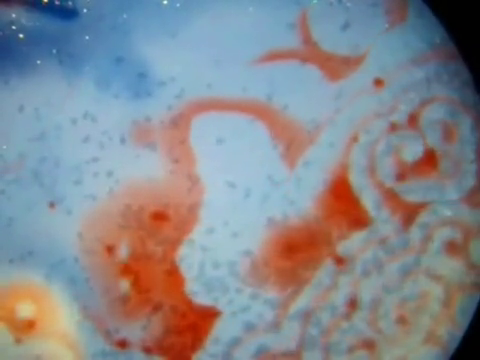
\includegraphics[scale=0.25]{BZ-frames0022.png}
% 
\includegraphics[scale=0.25]{BZ-frames0023.png}

\begin{comment}
% This fails because Linux's latest Acrobat Reader doesn't support SWF
% But it may work in Windows / Mac
\includemedia[
  width=0.4\linewidth,
  height=0.3\linewidth,
  activate=pageopen
]{}{BZ-movie.swf}
\end{comment}

\begin{figure}[ht]
\centering
\includemovie[label=BZ-movie,inline=false,text={
\includegraphics[scale=0.25]{BZ-movie-play.png}}]{}{}{BZ-movie.mp4}
%\caption*{BZ-reaction \movieref[pause]{BZ-movie}{Run}}
\end{figure}

想说的大概就那么多,其馀都是细节而已。

还有,我所讲的「世界 A 和世界 B」,其实差不多是同一个世界,亦即你和我活在其中的世界。 疯人院外面和里面的人没有分别。 我们每天都活在种族歧视之中、每天都互相出卖。 假设我在真人骚里而懵然不知,也不会有人道破这谎言。 他们只会对白人低着头「饶命啊大人」那个样子。 你们就是那些演员。

《圣经》里,\uline{摩西}想带\uline{以色列}人走出\uline{埃及},但初时人们反对他,说什么「我们现在做奴隶做得好好的,为什么要走?」 在《Waiting for Godot\footnote{等待果陀 (1953)}》剧里有个人像只狗那样被人用绳索拖着四脚走动,主角想解开他反被他咬。 据说 Che Guevara\footnote{(1928-1967)}帮助非洲人打游击战,被当地士兵的散漫态度弄到心力交瘁; Byron\footnote{(1788-1824)}也试图帮助希腊独立战争,因军队的士气低落而过劳致死。 那个叫「\uline{耶稣}」的人,也是在类似的情况下被人出卖而死的。 还有太多这样的例子.... ( ? )

我常想起\uline{耶稣}钉十字架时身旁的两个小偷,他们说『你既然是神的儿子,为什么落得和我们一样下场?』 我的目的就是要不死。

\begin{center}
\dashh 完 \dashh \par


\includegraphics[scale=0.5]{vignette0.jpg}
\end{center}

\chapter*{附录 A ~~~ 关於精神科药物}
\addcontentsline{toc}{chapter}{附录 A ~ 关於精神科药物}

实在有太多精神科药物的受害者,我觉得要写篇比较详细的解释,不用每次重复。

首先,人脑是靠这些神经细胞来思考的:
\begin{figure}[H]
\centering
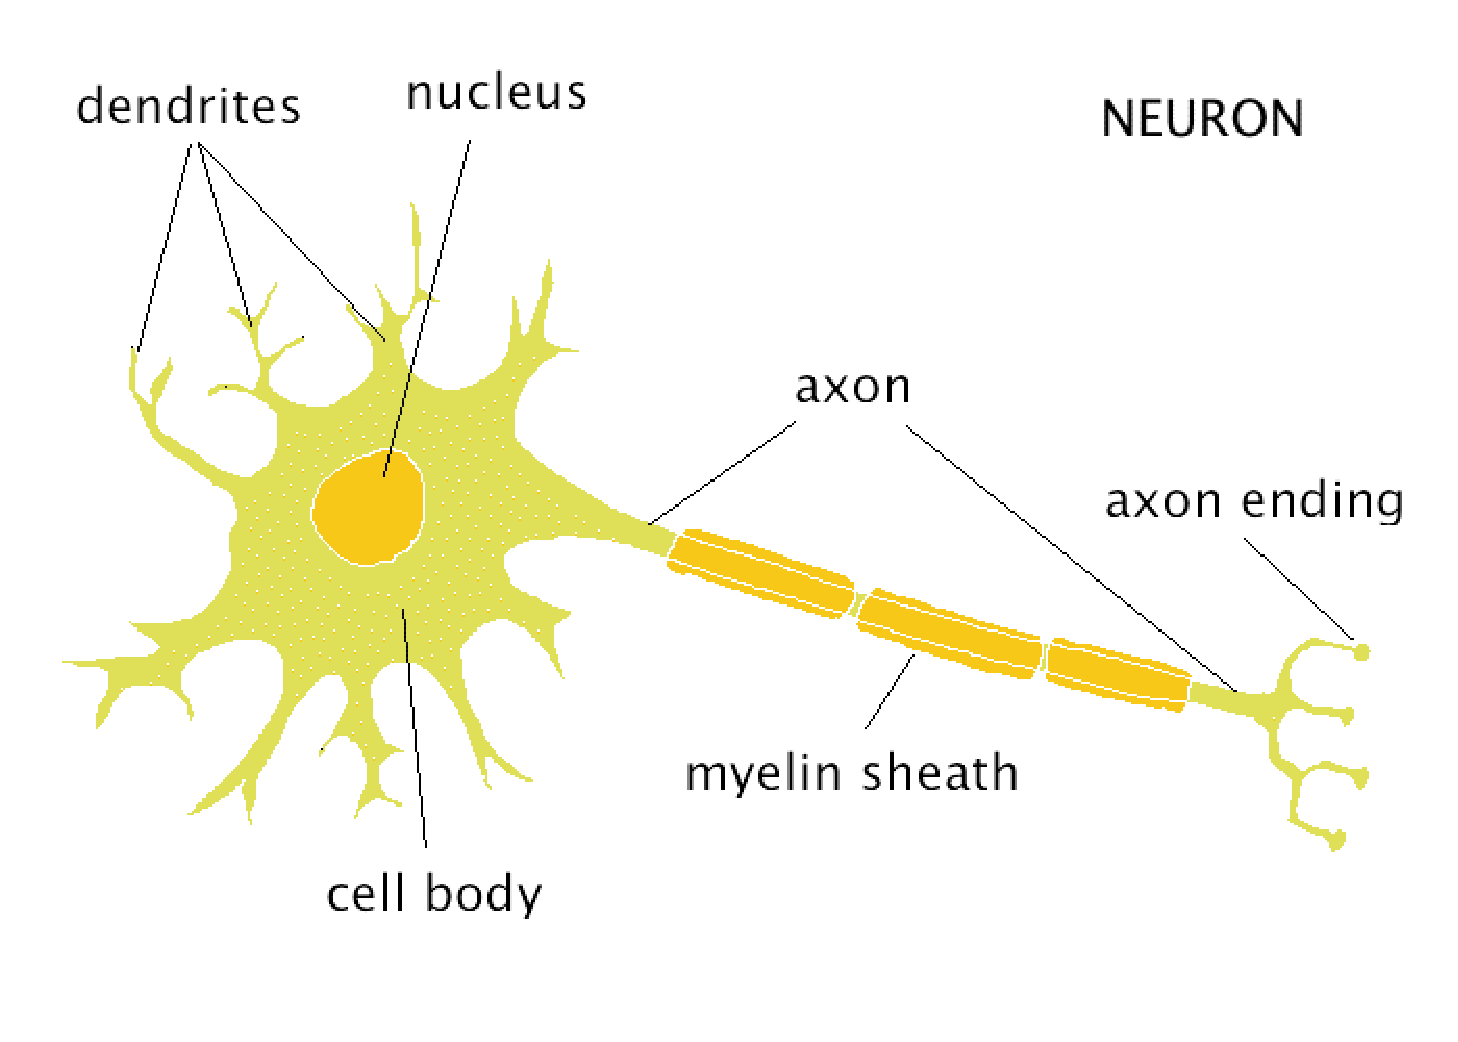
\includegraphics[scale=0.4]{neuron.pdf}
\end{figure}

每个神经细胞,由 dendrites 收集讯号,处理讯息后,经由 axon 传到别的神经细胞。 那些讯号是电讯号,有点像在电脑里面的情况。

人的喜怒哀乐、意识、思维、感觉、等,都是由这些神经讯号的运算产生的。 所以,脑死亡后便再没有意识,死亡就像灯的熄灭。

这是显微镜下(染了色)的神经细胞:
\begin{figure}[H]
\centering
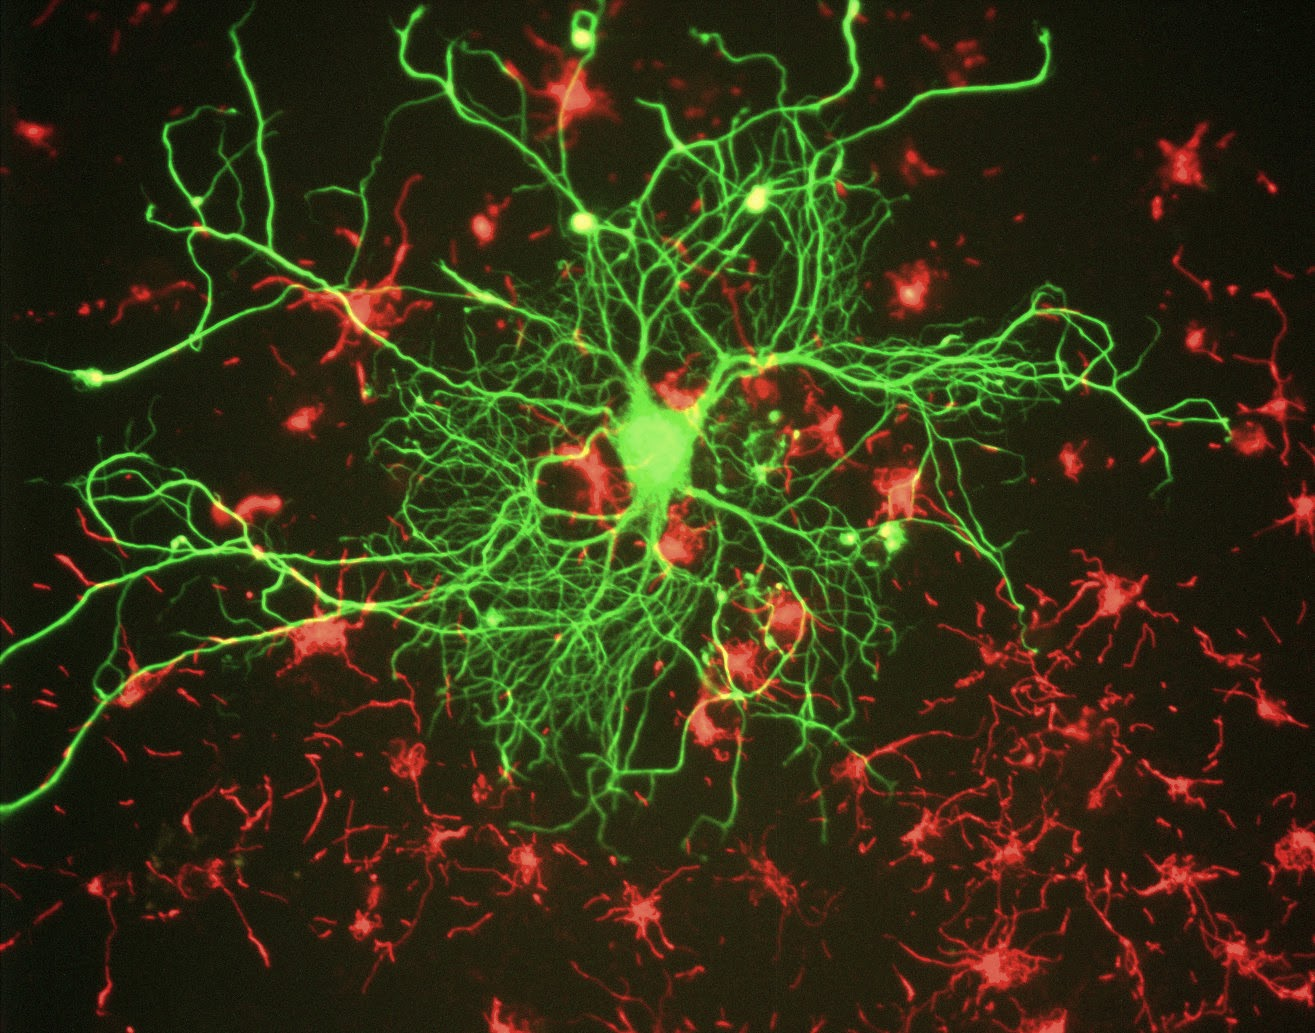
\includegraphics[scale=0.25]{neuron_in_tissue_culture.jpg}
\end{figure}

神经细胞之间的接点,叫 synapse「凸触」; 电讯号传到接点,便要靠一些化学分子来传递,它们即 neurotransmitter 「神经传播分子」。

精神科药物的原理,就是阻碍这些分子的传递 (blocking)。

例如,有一种神经传播分子叫 serotonin (血清素),「开心药」就是靠提升这分子而令病人的心情变好。

另一个神经传播分子是 dopamine,它负责人的动机和欲望,有很多控制精神分裂 (「发疯」) 的药物就抑制这个分子。 吃了,人会失去动机,连性欲也无,变得无精打彩,所以你们见精神病院里,那么多人像发呆似的行尸走肉。

人脑是一个很复杂的结构: 大脑分为很多区域 (brain areas); 大脑皮层有神经细胞,而脑中的白色物质是皮层之间的连线。 这些区域之间的连线图,可能比\uline{伦敦}地下铁图复杂几百倍,我们现在有没有这幅详细地图都成问题。 而,单是那皮层 (已经很薄) 也分为 6 层,每层之间有反覆的连络,其结构为什么如此,至今仍是一个谜。 脑里的神经细胞是地球人口的数十倍。 单一个神经细胞如何处理讯号? 那需要靠电流的微分方程解释。 而每个细胞又有成千上万的「突触」接收讯号。 更糟的是,那些化学信号的传播分子,种类也可能有几百以上,究竟有几多种还是未知之数。 刚才说的 serotonin 和 dopamine,只不过是最多见的那几种; 它们令到每个讯号都可能有性质上的不同。 这起码算概括了大脑的复杂性的规模。

简言之,科学家们根本弄不清人脑是如何思考; 距离这目标,我们还起码差几个\uline{诺贝尔}得奖者的努力,甚至那也是保守估计!

我们现时有些很笼统的知识,例如: serotonin 是「开心」、dopamine 是「动机」、某些地区例如 hippocampus 负责记忆、amygdala 负责感情 (如恐惧)、别的地区负责语言、视觉、等。

这些笼统的知识根本无法详细解释人们为什么有各式各样的精神病。

再看这是 serotonin 和 dopamine 在脑中的分布:
\begin{figure}[H]
\centering
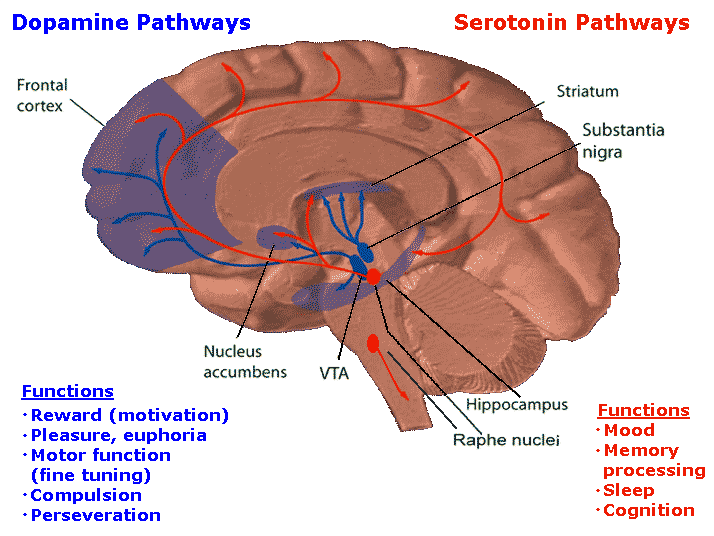
\includegraphics[scale=0.4]{dopamine_serotonin.png}
\end{figure}

早期的药物会把 (例如) 所有 dopamine 的接收都阻塞,但新药物能把某一特类 (sub-type) 的 dopamine 接收器阻塞。 但究竟每一类 dopamine 接收器的作用是什么? 我们不太明了。 那些所谓精神科药物的「专家」,就是在病人身上试试阻塞这个、阻塞那个、看看有什么反应。 你说可不可悲?

而且,由於正常的神經系統也會被阻塞了,那些服藥的病人通常是會較不服藥早死的。 例如他們會手震得很厲害,像心臟衰竭的老人。 而且吃了藥之後會坐立不安,是因為身體對這些「毒素」自然的抗拒反應; 很多病人會不斷喝茶,以沖淡藥的作用。 醫生有時會把藥打在病人臂部,那就不能不吃藥。 這樣的折磨本身就已經會令病人精神崩潰。

腦即思想和意識; 能夠控制別人的意識,那是神一般的能力。 有權力就會產生對權力的濫用 (abuse)。

也有些家庭,親人之間互相憎厭的時候就把較弱勢的一方送進精神病院。

破壞別人的腦就等於把那人作為「人」的本質毀滅。

人有各种各样的发疯,有些是先天性的,有些是后天的际遇刺激而起,也可以先天再加后天触发。

有些人遭遇很多不幸: 或者容貌特醜、被人欺壓、欺騙、歧視、被愛人拋棄、或各式各樣的不公平。 他們已經是受害者,還要被加害。

我们俗语常说「你快把我弄疯了」、「爱你爱到发疯」、那正表示某些际遇和感情是会导致精神病的; 但现代精神科 (psychiatry) 把一切解释成「脑内化学的不平衡」,仿佛病人的人生经历是无关的,连常识也违反 —— 这是发什么神经? 无非是贪钱而已。

在\uline{美国},精神病药厂每年赚很多亿\uline{美}元,而且他们直接赞助医生们,所以医生开那些药便可以赚多些钱。 药厂也赞助研究,发表对那些药的销售有利的研究结果。 甚至药物管理局 (FDA) 也可以用钱买通; 举例来说,帮小\uline{布殊}总统策划\uline{伊拉克}战事的 Donald Rumsfeld,他从商时曾经为公司帮政府通过以 aspartame 代糖取代 saccharin 代糖,但其实 aspartame 更差,吃多了会头痛\footnote{http://www.rense.com/general33/legal.htm}。 这就是\uline{美国}的资本主义。

最后,解释一下我知識的來源: 我先前研究过如何将人脑的「意識」上载到电脑上 (mind uploading),所以对神经科学很熟悉。 這是我的一些藏書:

\begin{figure}[H]
\centering
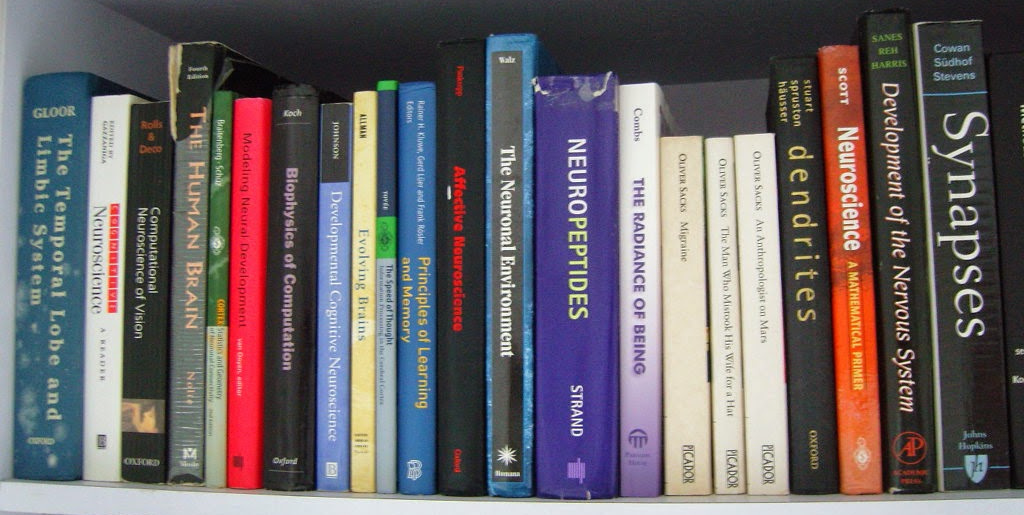
\includegraphics[scale=0.5]{neuro-books1.jpg}
\end{figure}

\begin{figure}[H]
\centering
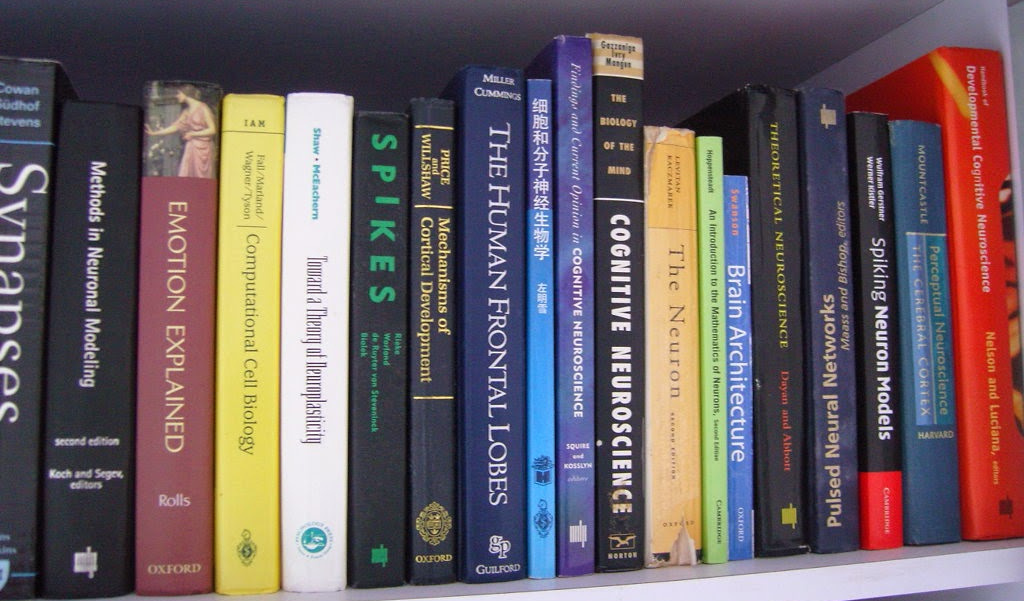
\includegraphics[scale=0.5]{neuro-books2.jpg}
\end{figure}

\begin{figure}[H]
\centering
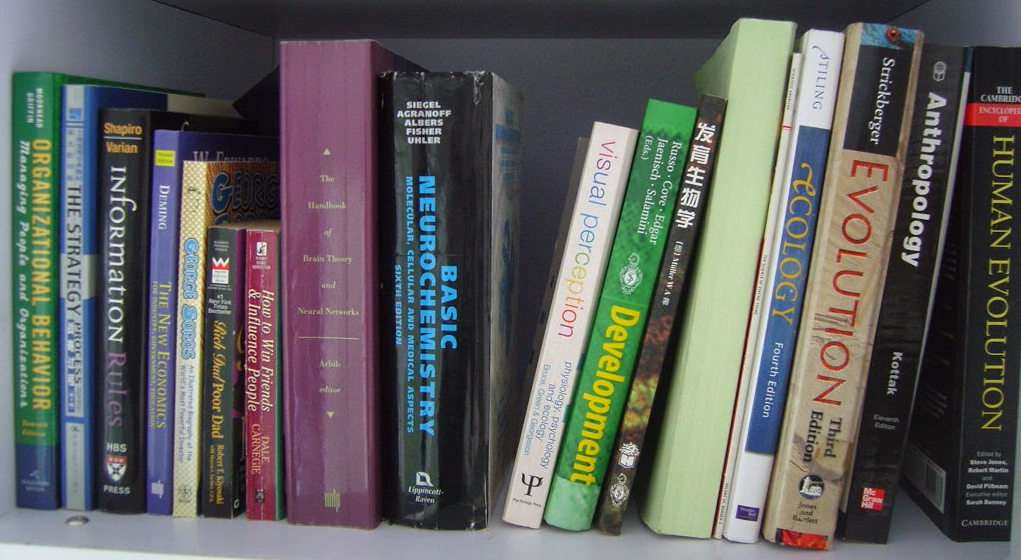
\includegraphics[scale=0.5]{neuro-books3.jpg}
\end{figure}

但自 2004 年我開始轉而研究人工智能,因為那技術的影響將會更厲害,大腦之謎也會間接地迎刃而解。

希望這篇文章能幫到我的病友們。

\chapter*{Acknowledgments}
\addcontentsline{toc}{chapter}{Acknowledgements}

( Apologize to relatives and friends.... )

%\bibliographystyle{plain} % or number or aaai ...
%\bibliography{AGI-book}

\onecolumn

% Bigger figures

\end{document}
